%
% File eacl2017.tex
%
%% Based on the style files for ACL-2016
%% Based on the style files for ACL-2015, with some improvements
%%  taken from the NAACL-2016 style
%% Based on the style files for ACL-2014, which were, in turn,
%% Based on the style files for ACL-2013, which were, in turn,
%% Based on the style files for ACL-2012, which were, in turn,
%% based on the style files for ACL-2011, which were, in turn, 
%% based on the style files for ACL-2010, which were, in turn, 
%% based on the style files for ACL-IJCNLP-2009, which were, in turn,
%% based on the style files for EACL-2009 and IJCNLP-2008...

%% Based on the style files for EACL 2006 by 
%%e.agirre@ehu.es or Sergi.Balari@uab.es
%% and that of ACL 08 by Joakim Nivre and Noah Smith

\documentclass[11pt]{article}
\usepackage{eacl2017}
\usepackage{times}
\usepackage{url}
\usepackage{latexsym}
\usepackage{listings}
\usepackage{graphicx}
\usepackage{rotating}

%\eaclfinalcopy % Uncomment this line for the final submission
%\def\eaclpaperid{***} %  Enter the acl Paper ID here

%\setlength\titlebox{5cm}
% You can expand the titlebox if you need extra space
% to show all the authors. Please do not make the titlebox
% smaller than 5cm (the original size); we will check this
% in the camera-ready version and ask you to change it back.

\newcommand\BibTeX{B{\sc ib}\TeX}

\title{Distant supervision for emotion detection exploiting Facebook reactions}

\author{First Author \\
  Affiliation / Address line 1 \\
  Affiliation / Address line 2 \\
  Affiliation / Address line 3 \\
  {\tt email@domain} \\\And
  Second Author \\
  Affiliation / Address line 1 \\
  Affiliation / Address line 2 \\
  Affiliation / Address line 3 \\
  {\tt email@domain} \\}

\date{}

\begin{document}
\maketitle
\begin{abstract}
  This document contains the instructions for preparing a camera-ready
  manuscript for the proceedings of EACL-2017. The document itself
  conforms to its own specifications, and is therefore an example of
  what your manuscript should look like. These instructions should be
  used for both papers submitted for review and for final versions of
  accepted papers.  Authors are asked to conform to all the directions
  reported in this document.
\end{abstract}

\section{Introduction}
Sentiment analysis is a term used for a broad range of Natural Language Processing (NLP) tasks, but most commonly this term is used for the task of detecting the polarity or valence in a piece of text. In most cases the classes \texttt{positive, neutral or negative} are used \cite{SentimentEmotionSurvey2015}. Some researchers use the term for a broader task, detecting emotions (i.e.  \texttt{anger, joy, fear, surprise, sadness and disgust}) and feelings in text. Both tasks are increasingly popular research areas due to the fact that an increasing amount of data is available via social media. This information can be useful for understanding how people feel about a certain topic, or to discover what mood the user is in. This information can for example be used to apply a different advertising strategy to an angry user than when the user is happy. It also can be used for detecting the opinion of people about something, for example how civilians think about the police after several shootings in 2016.\\\\
Some use-cases for automatically detecting emotions are described below \cite{SentimentEmotionSurvey2015}.
\begin{itemize}
\item Public health care; e.g. robots that can detect the patients emotion
\item Politics; e.g. predicting results using the stance towards candidates
\item Brand management; e.g. what do people think of your brand or product
\item Education; e.g. what is the influence of the mood of students while doing an exam.
\end{itemize}
One way to detect the emotion in a piece of text is training a model that can detect traits of a emotion, so called supervised learning, where a model is trained on a large amount of manually annotated examples. Using supervised learning for emotion detection has the disadvantage that a large corpus of annotated data is needed. Annotation is time consuming and in the case of emotion also difficult \cite{kim2010evaluation}. The emotion derived from a piece of text sometimes depends on the interpretation of the reader, making it difficult to be consistent in annotation. Some examples why it is difficult to annotate can be found in the next paragraph. Because of these reasons most researches focus on unsupervised techniques \cite{kim2010evaluation} and only a few on supervised techniques. Unsupervised approaches focus mainly on exploiting emotion lexicons. Both techniques were evaluated in the research by \cite{strapparava2008learning}, the results can be found in the evaluation section.\\\\

\subsection{The difficulty in detecting emotion in text}
Detecting emotion in text is a difficult task due to the complexity of language. Most language, especially on social media, is full of creativity in the form of metaphors, analogies, expressions of sarcasm, statements of irony, and so on. In the NLP community this is referred to as figurative language. Some examples from the the SemEval 2007 shared task, where contenders where asked to build a system that can classify headlines in six emotions (\texttt{anger, disgust, fear, joy, sadness} and \texttt{surprise}), illustrate the difficulty in classifying emotions.
\begin{lstlisting}
"Apple drops bombshell with iPhone"
\end{lstlisting}
This headline is easy to classify for a human because because most people will understand the semantic meaning of this sentence, knowing what an iPhone is and therefore understanding that Apple refers to a company and not to a fruit. By contrast this sentence is difficult to classify for a computer because it does not understand the semantic meaning of the words in the sentence. Just looking at the words used this could be seen as a negative sentence, but in reality it is about something positive. \\\\
Also a mix of positive and negative words makes it difficult for a model to classify sentences.
\begin{lstlisting}
"Spain ahead although Nadal is out"
\end{lstlisting}
The last example also shows the difficulty in annotating, the process of manually labeling the corresponding emotion to each sentence that can be used to train a model. You could argue that the main emotion is positive because the Spanish team is ahead to the next round but the star-player Nadal is out. If multiple people where asked to annotate this headline you could expect different answers, therefore for a computer it is also difficult. 

\subsection{Research question}
As mentioned, supervised learning has the disadvantage that a large set of annotated data is needed to train a model. In this thesis I explore the possibility to use automatically collected data from Facebook to train an emotion classification model.\\\\
Facebook enables users to respond to a post with an emotion. This emotion feature was introduced in February 2016 and was an addition to the well-known like button. Facebook introduced it so people had more options to quickly respond to a post, e.g. to respond to a sad post users can respond with a sad smiley instead of the Like button.\\\\
In this research I want to download posts from several Facebook Pages and for each post retrieve the count per reaction type. Idea is that if the majority emotion reaction is \texttt{angry} the post is labeled with the \texttt{angry} class. Interesting will be if the results by using Facebook data and evaluated on some manually annotated data-sets will yield similar or better results as compared to systems that are trained and tested on the same manually annotated data. The approach of using Facebook data can be seen as semi-supervised learning since the annotation is done by people but not with the goal of training a model.\\
\begin{figure}
  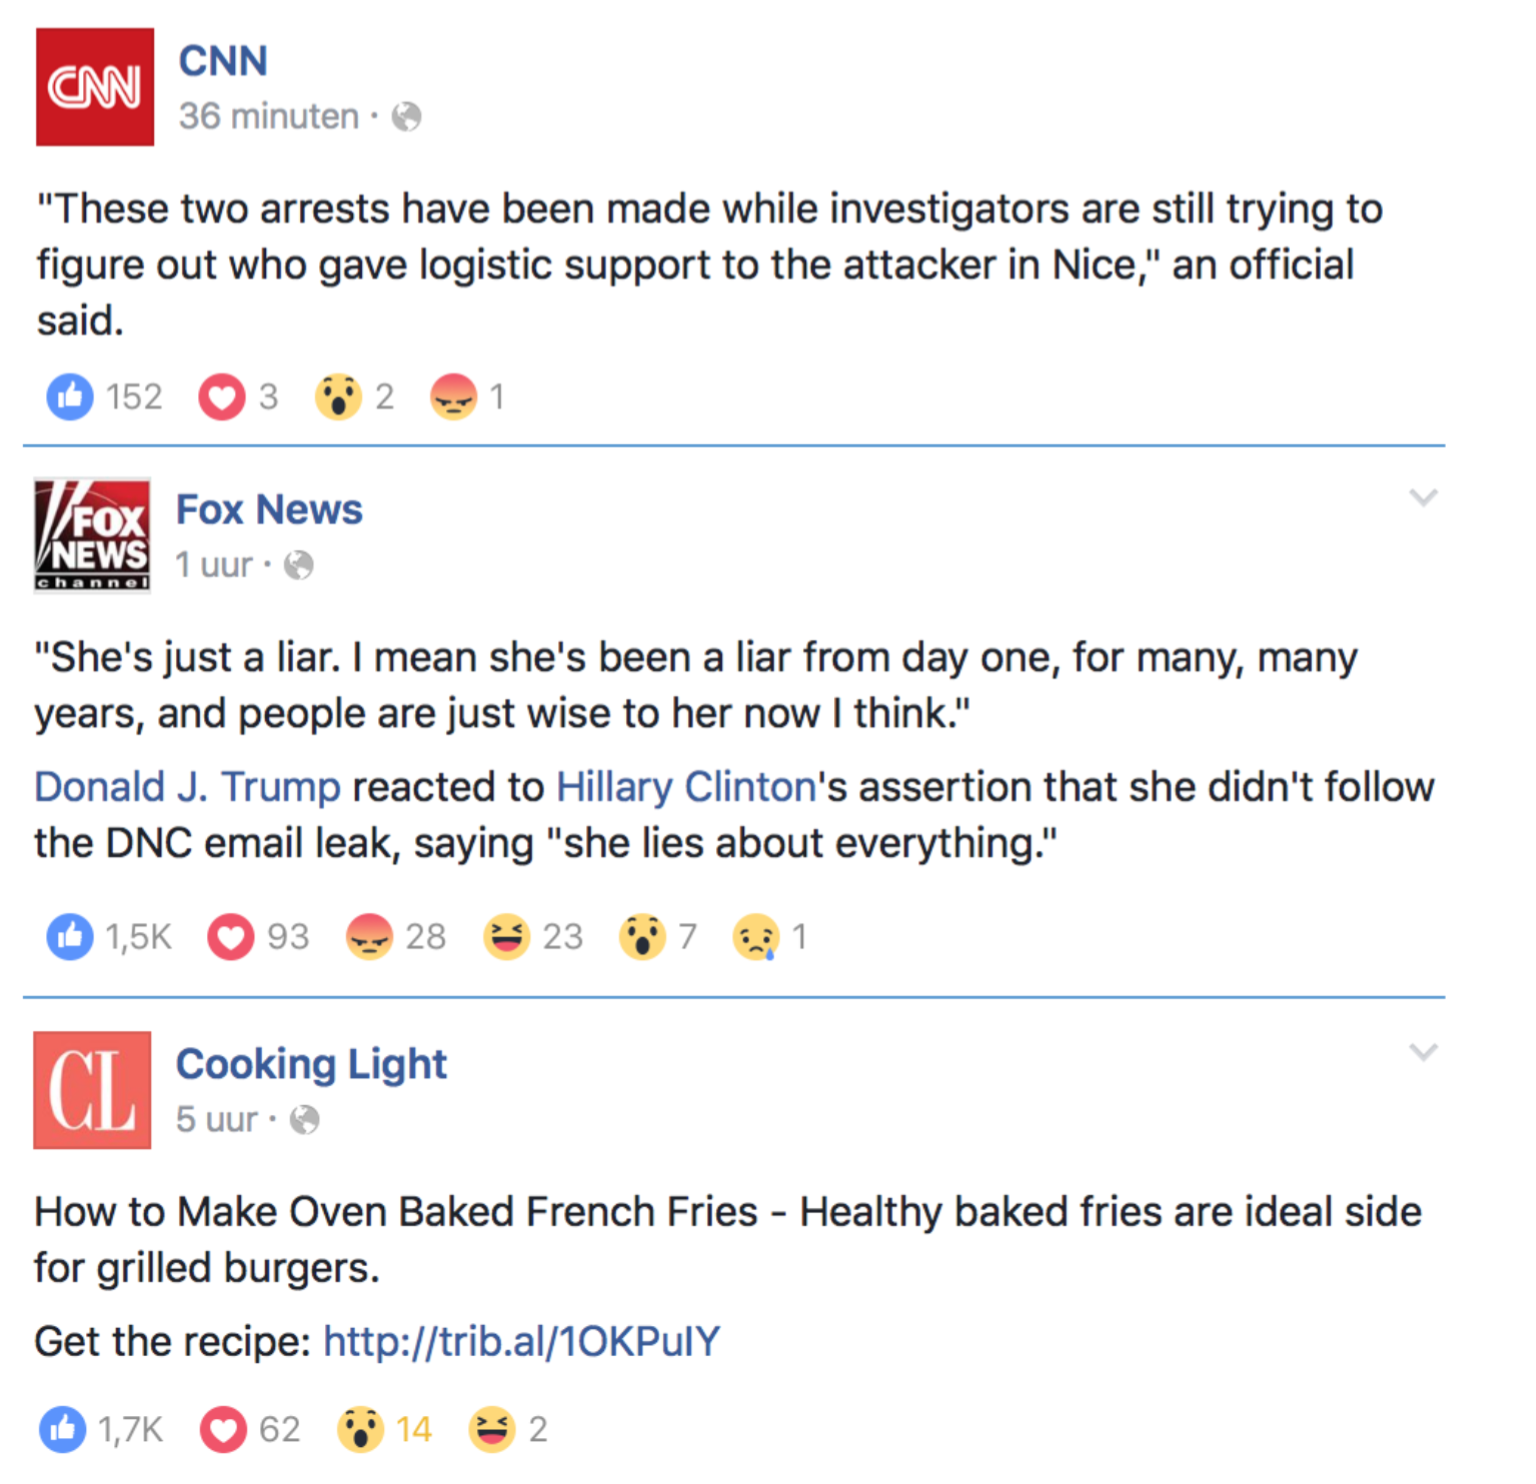
\includegraphics[width=\linewidth]{example_posts.png}
  \caption{Posts on Facebook}
  \label{fig:example_facebook_posts}
\end{figure}\\
In figure \ref{fig:example_facebook_posts} some example Facebook posts can be found from different Facebook pages with the count of emotions mentioned. An interesting finding is that on the post from \texttt{FoxNews} people respond with quite diverse emotions, probably because some people are in favor of \texttt{Donald Trump} and some are in favor of \texttt{Hillary Clinton}. This also illustrates that it is important to make a good balanced set of Facebook pages to train a model on and that the retrieved label does not always reflect the content of the post but in some cases the emotion of the reader.

\subsection{Proposed method}
For this research I want to train a model using the automatically harvested data from Facebook described in section section three. For evaluation I will use the data-sets described in section four. For creating the model I will use Python and Scikit learn \cite{scikit-learn}, these tools provide a lot of features helpful in developing a system. For the final results I want to compare my system with others that have evaluated their systems on the same data-sets. An overview of this method can be found in figure \ref{fig:proposed_method}
\begin{figure}[ht]
  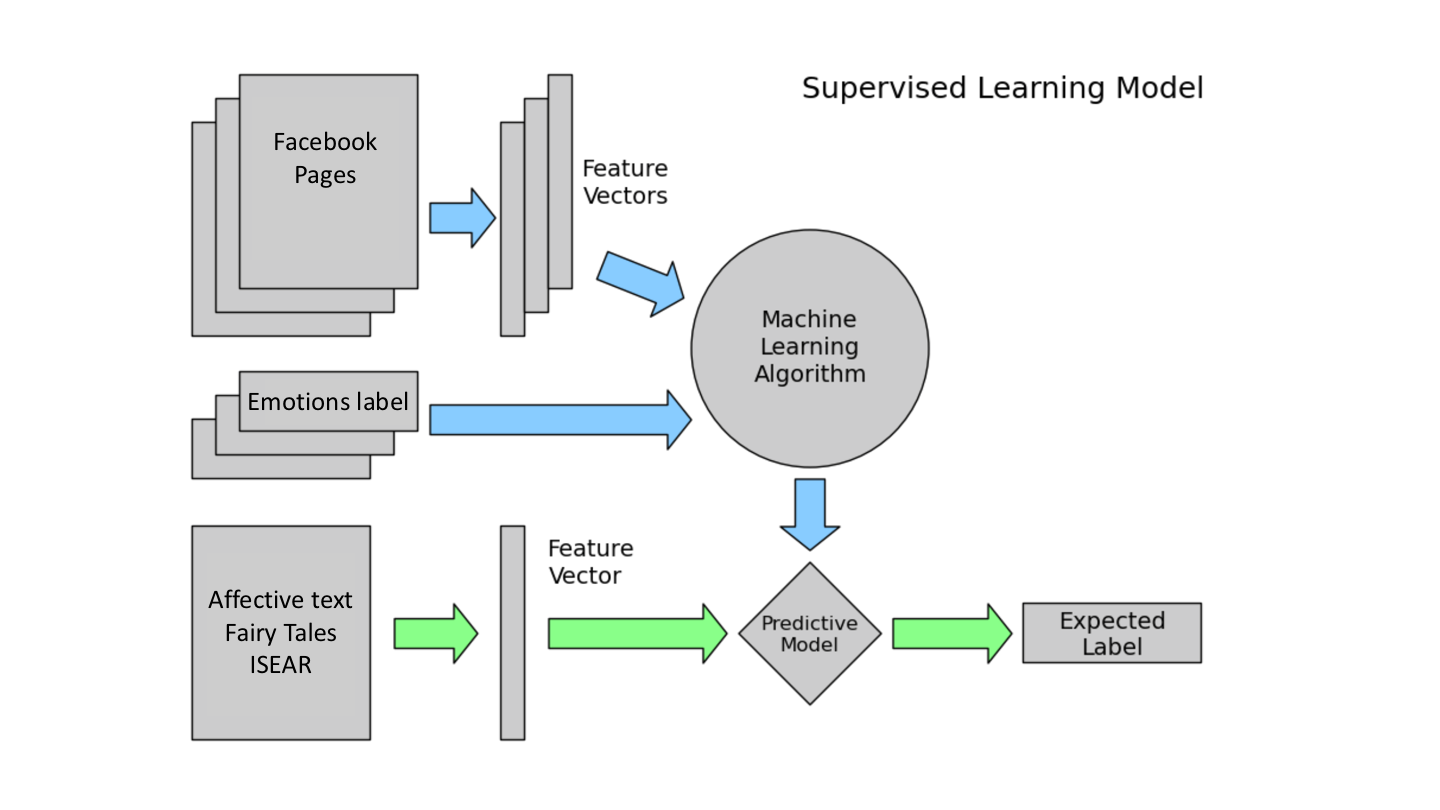
\includegraphics[width=\linewidth]{supervised_learning.png}
  \caption{Proposed method \cite{astroMLText}}
  \label{fig:proposed_method}
\end{figure}\\

\subsection{Project structure}
This thesis was created using \LaTeX  and can be found together with all scripts used on my GitHub page\footnote{www.github.com/chrispool}.



\section{Related work}
In this chapter, an overview is given on existing research on emotion detection. This section gives some more background information that can be helpful in my experiment.

\subsection{Emotion models}
There are two different models for representing emotions, the \textit{categorical model}, e.g. Ekman\'s six emotions\cite{ekman1992argument} and the \textit{dimensional model} \cite{russell2003core}. The categorical model is an approach where there are a number of primary and unrelated emotions. \newcite{ekman1992argument}'s basic emotions are \texttt{Anger, Disgust, Fear, Joy, Sadness} and \texttt{Surprise} and is a good example of a categorical model where each emotion is characterized by some features that induce certain responses  or conditions. \\\\
The dimensional method represents emotion in a dimensional form. where emotion are related by a common set of dimensions (e.g. valence or arousal) and are generally defined in a two or three dimensional space \cite{mohammad2015sentiment}. Each emotion occupies some location in this space. A valence dimension indicates positive and negative emotions on different ends of the scale. The arousal dimension differentiates excites vs. calm states. An example can be found in figure \ref{fig:circumplex}.

\begin{figure}[ht]
  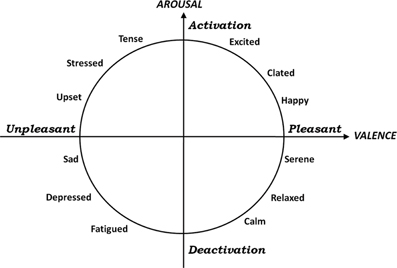
\includegraphics[width=\linewidth]{5425219.jpg}
  \caption{Circumplex Model of Affect}
  \label{fig:circumplex}
\end{figure}



\subsection{Sentiment analysis}
Sentiment Analysis is used for a broad range of related but different problems. In most cases the term Sentiment Analysis is used for automatically determining the polarity of a piece of text, so if the text is about something positive or negative, and in some cases neutral. The Circumplex model as shown in figure \ref{fig:circumplex} has two primary dimensions, the Valence and arousal dimension making it not surprising that large amount of research focuses on determining valence in text \cite{pang2005seeing}.\\\\
Detecting the valence of a piece of text is interesting because most people are interested in the opinion of other people before buying a product, going to a restaurant etc. \cite{pang2008opinion}. Also knowing political information is for a large group of people interesting. With ever increasing amounts of data about products, companies and persons available on social media the need to automatically derive the sentiment is useful.\\\\
For detecting the valence of a piece of text machine learning is a common approach. For this task numerous of annotated data-sets are available, some of the most used data-set is the Movie Review data-set \cite{pang2002thumbs} where each movie has a binary label, 1 being positive and 0 being negative. The advantage of this approach that data-sets can relatively easy be collected, in the case of the movie-review data-set the ratings, for example a scale from 1-5 can be used to create a label (1,2 being negative, 3 is ignored and 4 and 5 being positive). Also some experiments have been done using Twitter, a tweet with a sad emoticon is used as a negative example and a tweet with a happy emoticon used as a positive example \cite{mohammad2015using}.

\subsection{Affect classification}
Detecting affect in text is a much harder task and only in interest of researches the last years. This is probably due to the increasing interest and availability of data. Most research is focused on classifying using \newcite{ekman1992argument}'s six basic emotion. But also some work had done in using more complex emotion models.


\subsubsection{Unsupervised vs supervised}
Because there are hardly any data-sets for affect classification to use as train data most approaches are unsupervised. Meaning no training-data is needed and other resources are used for determining the emotion in a piece of text. For example using lexicons, described in \ref{lexicon_section}. Some supervised approaches (\cite{chaffar2011using}, \cite{kim2010evaluation}) achieve good results but are very domain specific.


\subsubsection{Lexicons}
\label{lexion_section}
Lexicons is used in most researches, most lexicons contain information about words and the corresponding emotion.
\begin{description}
\item[Wordnet affect lexicon] Few thousand words with a number of affect categories associated \cite{strapparava2004wordnet}.
\item [NRC 10] Few thousand words with a number of affect categories associated \cite{mohammad:2012:NAACL-HLT}.
\end{description}
Lexicons have proven to be quite successful in detecting emotions in text, the work done by \newcite{mohammad:2012:NAACL-HLT} can be useful for developing my system.


% \subsection{Social media data-sets}


% \subsection{Facebook reactions}
% How do people use Facebook reactions

% \paragraph*{Sentiment Analysis: Detecting Valence, Emotions, and Other Affectual States from Text. Saif M. Mohammad, Emotion Measurement, 2016. }
% http://saifmohammad.com/WebDocs/emotion-survey.pdf \cite{SentimentEmotionSurvey2015} \\
% Sentiment analysys can be used to refer to many different but related problems. It is mostly used to describe the polarity, (postive, negative or neutral). But more generally it refers to determing someones attittude towards a particular topic or target. The attitude could be an emotion like angry, sad, joy etc. In this book sentiment analysys is the task to retrieve the polarity and emotions in a text. The first part sums up research done in retrieving polarity and the strength of the polarity. \\\\
% Emotion detection can be usefull for several domains, for example automatic detection of bullying, in politics there is a huge interest in the sentiment of the public towards politicians. Companies are also interested what the attitude of their customers is. Students tend to learn better when the student is happy, emotions in social media, differences in gender, detecting persionaliyt traits, analysys of literature and visulazing emotions. \\\\
% Many shared tasks about sentiment analysis are organized by SemEval.
% THe book has a good description about why it is difficult to do sentiment analysus. Good starting point for the introdoction part of my thesis. In chapter 4.2 he describes several datasets that i can use.


% \subsection{To read}

% \cite{strapparava2008learning}


% \paragraph*{Emotional Tweets, Saif Mohammad, In Proceedings of the First Joint Conference on Lexical and Computational Semantics, June 2012, Montreal, Canada.}
% http://ixa2.si.ehu.es/starsem/proc/pdf/STARSEM-SEMEVAL033.pdf \cite{mohammad:2012:STARSEM-SEMEVAL}

% \paragraph*{Portable Features for Classifying Emotional Text, Saif Mohammad, In Proceedings of the 2012 Conference of the North American Chapter of the Association for Computational Linguistics: Human Language Technologies, June 2012, Montreal, Canada.}
% http://aclweb.org/anthology/N/N12/N12-1071.pdf \cite{mohammad:2012:NAACL-HLT}

% \paragraph*{Getting Emotional About News. Alistair Kennedy, Anna Kazantseva, Saif Mohammad, Terry Copeck, Diana Inkpen, Stan Szpakowicz. Proceedings of the Text Analysis Conference (TAC-2011), November 2011, Gaithersburg, MD.}
% http://www.nist.gov/tac/publications/2011/participant.papers/uOttawa.proceedings.pdf


% \subsection{Emotion detection using annotated corpora/lexicons}

% \paragraph*{Using a heterogeneous dataset for emotion analysis in text}
% \cite{chaffar2011using} is a paper about using three different datasets to train a model to detect emotions in text. This paper can be useful to compare my system with.
% % * <chrispool@gmail.com> 2016-07-26T13:43:18.263Z:
% %
% % ^.
% \paragraph*{Evaluation of unsupervised emotion models to textual affect recognition}
% \cite{kim2010evaluation} uses three data sets to evaluate several unsupervised models for detecting emotion in text. They make use of the SemEval, ISEAR and Fairy tales dataset that well be discussed in section 3. Because of the datasets they use it makes it possible to compare my system to theirs.


% \subsection{Emotion detection in Social media (generating train sets automatically or crowdsourcing)}
% \paragraph*{Emotex: Detecting emotions in twitter messages}
% Interesting paper about using tweets as automatic generated train data. They harvest tweets with hashtags that appear in the .. model. A model that has all the emotions and feelings between 

% \paragraph*{Using hashtags to capture fine emotion categories from tweets}
% Paper about emotion detection in social media \cite{mohammad2015using} Also a paper that describes a method to get emotions from twitter using the hashtags.

% \paragraph*{Semantic Role Labeling of Emotions in Tweets. Saif M. Mohammad, Xiaodan Zhu, and Joel Martin, In Proceedings of the ACL 2014 Workshop on Computational Approaches to Subjectivity, Sentiment, and Social Media (WASSA), June 2014, Baltimore, MD.}
% http://saifmohammad.com/WebDocs/whowhatwhom.pdf \cite{W14-2607} This paper describes a method of automatically compiling a dataset of tweets pertaining tot the 2012 us elections and not only the emotion but also who is feeling that emotion. They select the tweets using some seletecd hashtags and use crowdsourcing to annotate the tweets. They describe features for training a model for emotion detections and the performance.

% \paragraph{Sentiment, emotion, purpose, and style in electoral tweets}
% \cite{mohammad2015sentiment} describes a research about classifying sentiment in electoral tweets and describe the aspects what makes a electoral tweet a certain sentiment.
  
  
\newpage  
\section{Facebook reactions data-set}
Emotion annotated data sets are hard to find and annotation is an expensive and time-consuming task \cite{kim2010evaluation}. Facebook enables users to respond to posts using standard emotions. The standard reactions that can be used to respond to a post are \texttt{Like, Love, Haha, Wow, Sad and Angry} as can be seen in Figure \ref{fig:facebook_reactions}. This feature, introduced in 2016, can be seen as a form of annotation. Facebook posts and their corresponding reactions can be collected using the Facebook API. This enables to get domain specific examples by using different Facebook pages. These combinations of posts and the corresponding reactions can be used for training a emotion classifier by for example using the emotion most used as label. The advantage of this approach is that huge amounts of domain specific annotated data can be collected fairly easy. 

\begin{figure}[hbt]
  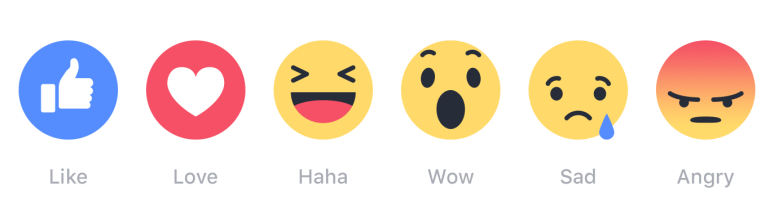
\includegraphics[width=\linewidth]{reactions-image-en_us.png}
  \caption{Facebook reactions}
  \label{fig:facebook_reactions}
\end{figure}

\subsection{Facebook reactions}
In February 2016 the Facebook reactions feature became available world-wide. This enables users to react to posts or photos with a certain emotion as can be seen in Figure \ref{fig:facebook_reactions}. Liking a post was for a long time the only possibility to respond to a post, but with this new feature it enables you to respond with the corresponding emotion. This new feature helps Facebook to know much more about their users, for example in what kind of mood a user is that can be used for advertising. \cite{wired} This information can also be seen as a form of annotation, users respond mostly about how a post makes them feel. Difficult is to interpret how the user uses this reaction, in some cases the emotion is about the post because the news is sad, happy etc. But in some cases it expresses a certain stance. For example the post in Figure \ref{fig:facebook_reactions_post_football} is about Chile beating Colombia in a football match during the Copa América. Some people respond to that information with a happy reaction and other people with a sad reaction depending the team you support, making that in some cases the reaction is a stance towards something and in some cases the reactions refer to the actual content.

\begin{figure}
  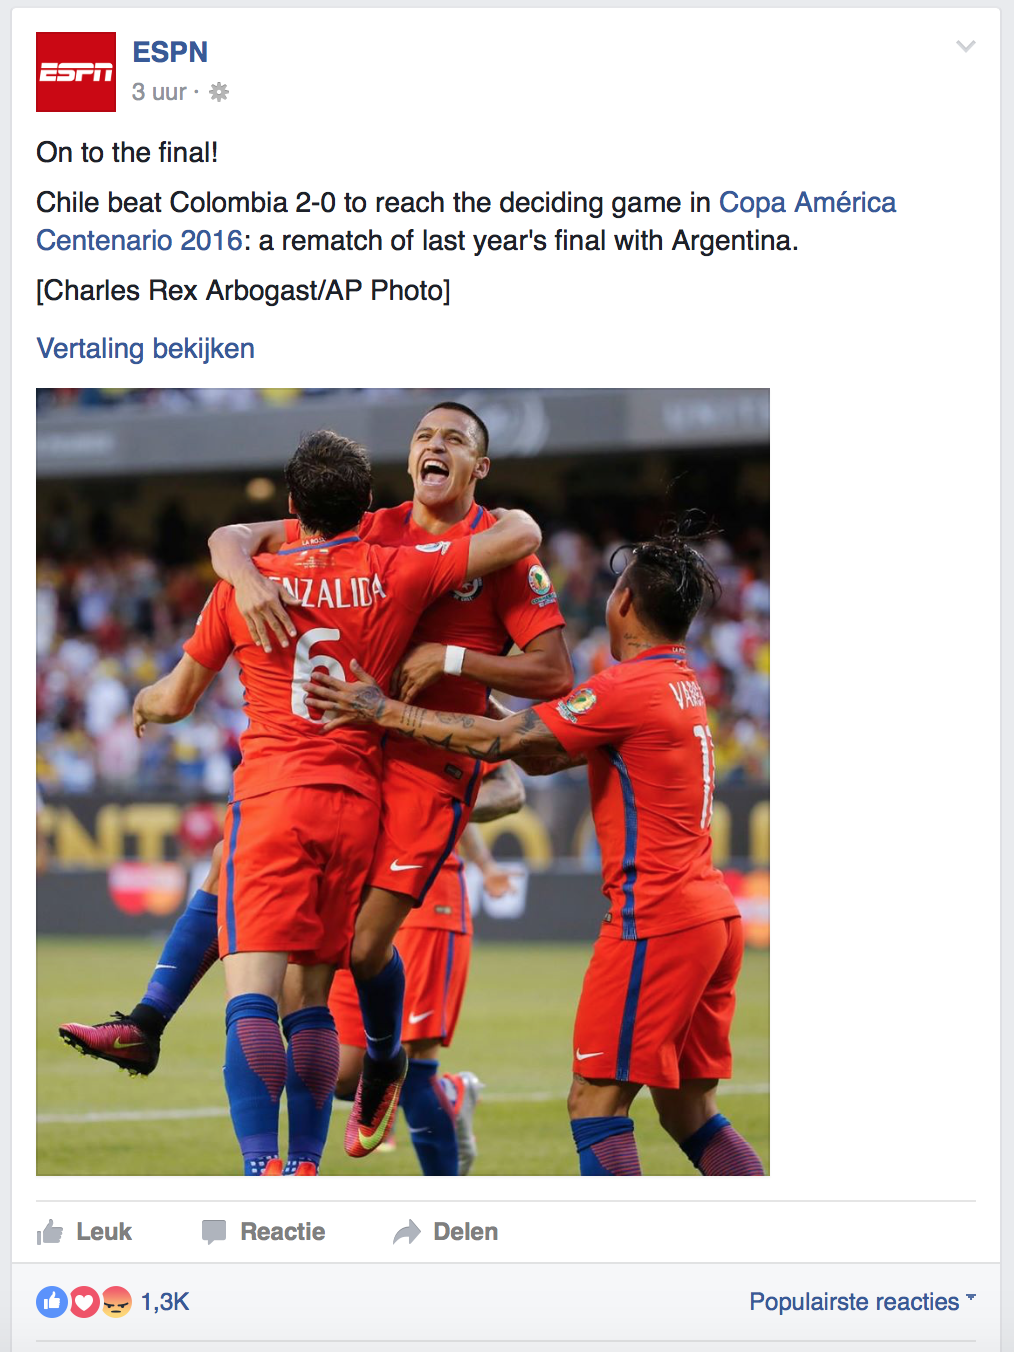
\includegraphics[width=\linewidth]{facebook_post_football.png}
  \caption{Post on Facebook}
  \label{fig:facebook_reactions_post_football}
\end{figure}

\subsection{Using the API}
The Facebook API enables developers to interact with data available on Facebook, depending on the permissions you have. Using the API requires a developers account that easily can be created on \verb+http://developers.facebook.com+. For getting my training data I created a script (get\_facebook\_reactions.py) that can be found in the GitHub repo. First it downloads the last 1000 posts if available since February 2016, the period Facebook started with the reactions. For my scripts I used the excellent Python Facebook library written by Martey Dodoo \footnote{https://pypi.python.org/pypi/facebook-sdk}. 

\begin{lstlisting}[language=Python, caption=Script that retrieves the posts from a Facebook page]
#download all posts from the CNN page
cnn_posts = get_all(graph.get_object(id="cnn/feed"))
for post in cnn_posts:
        
  try:
    # Perform some action on each post in the collection
    #  we receive from Facebook.
    cnn_posts.extend(items['data'])
    # Attempt to make a request to the next page of 
    # data, if it exists.
    items = requests.get(items['paging']['next']).json()
  except KeyError:
    # When there are no more pages break from the
    # loop and end the script.
    print("....Finished getting data")
    break
\end{lstlisting}
The snippet above retrieves the first 20 posts using the code on line 2. Each request to the API is limited to 20 items being returned but contains the url for the next 20 items. I use this url in a for loop, where I continue querying the webservice until there are no more pages available, resulting in a list of posts. \\\\
The second step is to retrieve the count of reactions for each post. Because the API does not enable you to get the count of all reactions I wrote a script that retrieves per post the count per emotion as can be seen in the snippet below.

\begin{lstlisting}[language=Python, caption=Retrieving emotion vector using Facebook API]
possible_reactions = ['NONE', 
                      'LIKE', 
                      'LOVE', 
                      'HAHA', 
                      'WOW', 
                      'SAD', 
                      'ANGRY', 
                      'THANKFUL']
for i, post in enumerate(cnn_posts):      
        if 'message' in post: #filter out events
            reaction_vector = []
            for reaction in possible_reactions:
                rs = graph.get_object(id="{}?fields=reactions.type({})
.summary(true)" .format(post['id'], reaction))
                                     
                reaction_vector.append(rs['reactions']['summary']['total_count'])
  
            result.append([{'created_time': post['created_time'], 
                            'message': post['message'], 
                            'reactions': reaction_vector}])
\end{lstlisting}
The final result list contains a list of dictionaries with a timestamp, message and a reaction vector. This is written to a JSON file as can be seen in the code example below.

\begin{lstlisting}[language=Python, caption=Example JSON data]
[
        {
            "created_time": "2016-06-19T01:40:00+0000",
            "message": "Walt Disney World representatives said
            they plan to put up fencing and signs at all resorts
            and waterways.",
            "reactions": [
                5073,
                4483,
                60,
                22,
                54,
                284,
                170,
                0
            ]
        }
    ],
    [
        {
            "created_time": "2016-06-19T01:00:00+0000",
            "message": "Charlene and Joseph Handrik face more
            than 550 counts of animal cruelty.",
            "reactions": [
                2256,
                1011,
                16,
                6,
                123,
                409,
                691,
                0
            ]
        }
    ],
\end{lstlisting}

\subsection{Permissions}
User pages also contain a lot of domain specific examples that can be used for training a classifier. Due to the privacy policy of Facebook it was not possible to collect these posts. This is only possible if the user key you use for the requests belongs to a friend of the person you want to retrieve the posts from \footnote{https://developers.facebook.com/bugs/290004301178437/}. 

\subsection{Choosing Facebook pages}
For my experiment I collected the posts from several Facebook pages from different domains to get a good balanced data set. I chose the pages primarily based on intuition. For the experiment I want to select the pages that are most similar to the target domain. The results per Facebook page and which pages I ended up using can be found in the Experiment section. In figure \ref{fig:distribution_facebook} you can find an overview of the distribution per Facebook page. \\\\
The distribution indicates that pages about news tend to have more sadness and anger posts where pages about cooking, tv-shows have a high percentage of joy posts. Depending on the target domain a combination of different pages can be used to get the best performance.
\begin{sidewaysfigure}
    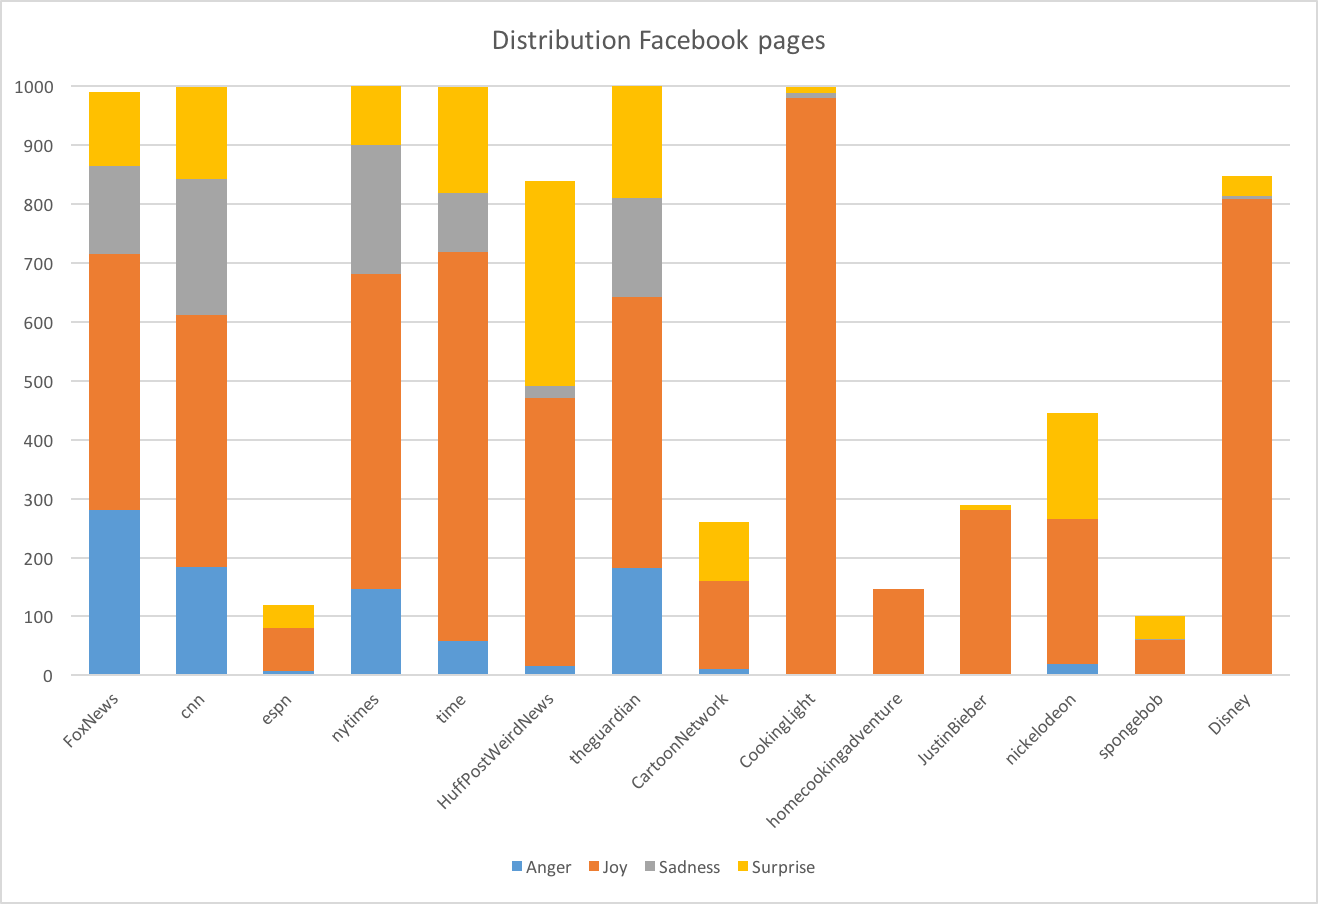
\includegraphics[width=\textwidth,height=\textheight,keepaspectratio]{distribution_facebook.png}  
\caption{Distribution of posts per page}
\label{fig:distribution_facebook}
\end{sidewaysfigure}



\section{Evaluation Datasets}
Three datasets annotated with emotions are commonly used for the evaluation of systems. We have used them, too so that we could evaluate the accuracy of our system and compare directly to other existing models. In this section we describe them, together with an explanation of how we mapped our emotion labels to those in the datasets, whenever necessary.

\subsection{Affective text dataset}
This data-set was created for the shared task were contenders where asked to classify emotions and valence in news headlines during SemEval 2007 \cite{strapparava2007semeval}. This task was designed to explore the connection between emotion and lexical semantics. The reason headlines where chosen is because  in most cases they contain only a few words and are written with the purpose to attract the readers attention. The headlines where collected from several news websites including Google news, New York Times, BBC News and CNN. \\ \\
The goal of the shared task was to classify each headline with the correct emotion class (i.e. \texttt{Anger, Disgust, Fear, Joy, Sadness, Surprise}) and to classify the valence (positive/negative). Classification of emotion and valence where seen as separate tasks. \\ \\
Data was annotated by giving a score from 0 to 100 for each emotion, making it possible to annotate a headline with multiple emotions. The data was annotated by six people
The data-set is divided in a development set consisting of 250 annotated headlines and a test set with 1.000 annotated headlines.
This data-set is used in several papers on the topic of emotion detection. For the original task, the shared task~\#14 at SemEval 2007, \cite{strapparava2007semeval} the evaluation was done using two different methods; the fine-grained evaluation was done by using the Pearson correlation measure between the system scores and the gold standard. The coarse-grained method was done by converting each emotion to a binary label. Because most papers use the coarse-grained method I also choose to convert the data to categorical labels.

In most researches, the vector of emotion was converted to a categorical label, in all researches the emotion with the highest value was used (\cite{chaffar2011using}, \cite{calvo2013emotions} and \cite{kim2010evaluation}).
In the paper by \cite{kim2010evaluation} they evaluated several unsupervised techniques using, among others, this data-set. The results, reported in precision, recall and f-score can be found in section 5. \newcite{strapparava2008learning} also used this data-set to evaluate five different unsupervised techniques . The results are also reported using precision, recall and f-score for each emotion category. \newcite{mohammad:2012:NAACL-HLT} uses this data-set for testing different supervised learning techniques and the portability of features \cite{mohammad:2012:NAACL-HLT}.

\paragraph{Technical description}
The data-set consists of four files. For the development and test-set both two XML files are used. One XML file contains the headlines with an ID, the other XML file contains the emotion vector (score for each emotion).
\begin{figure}[htb]
  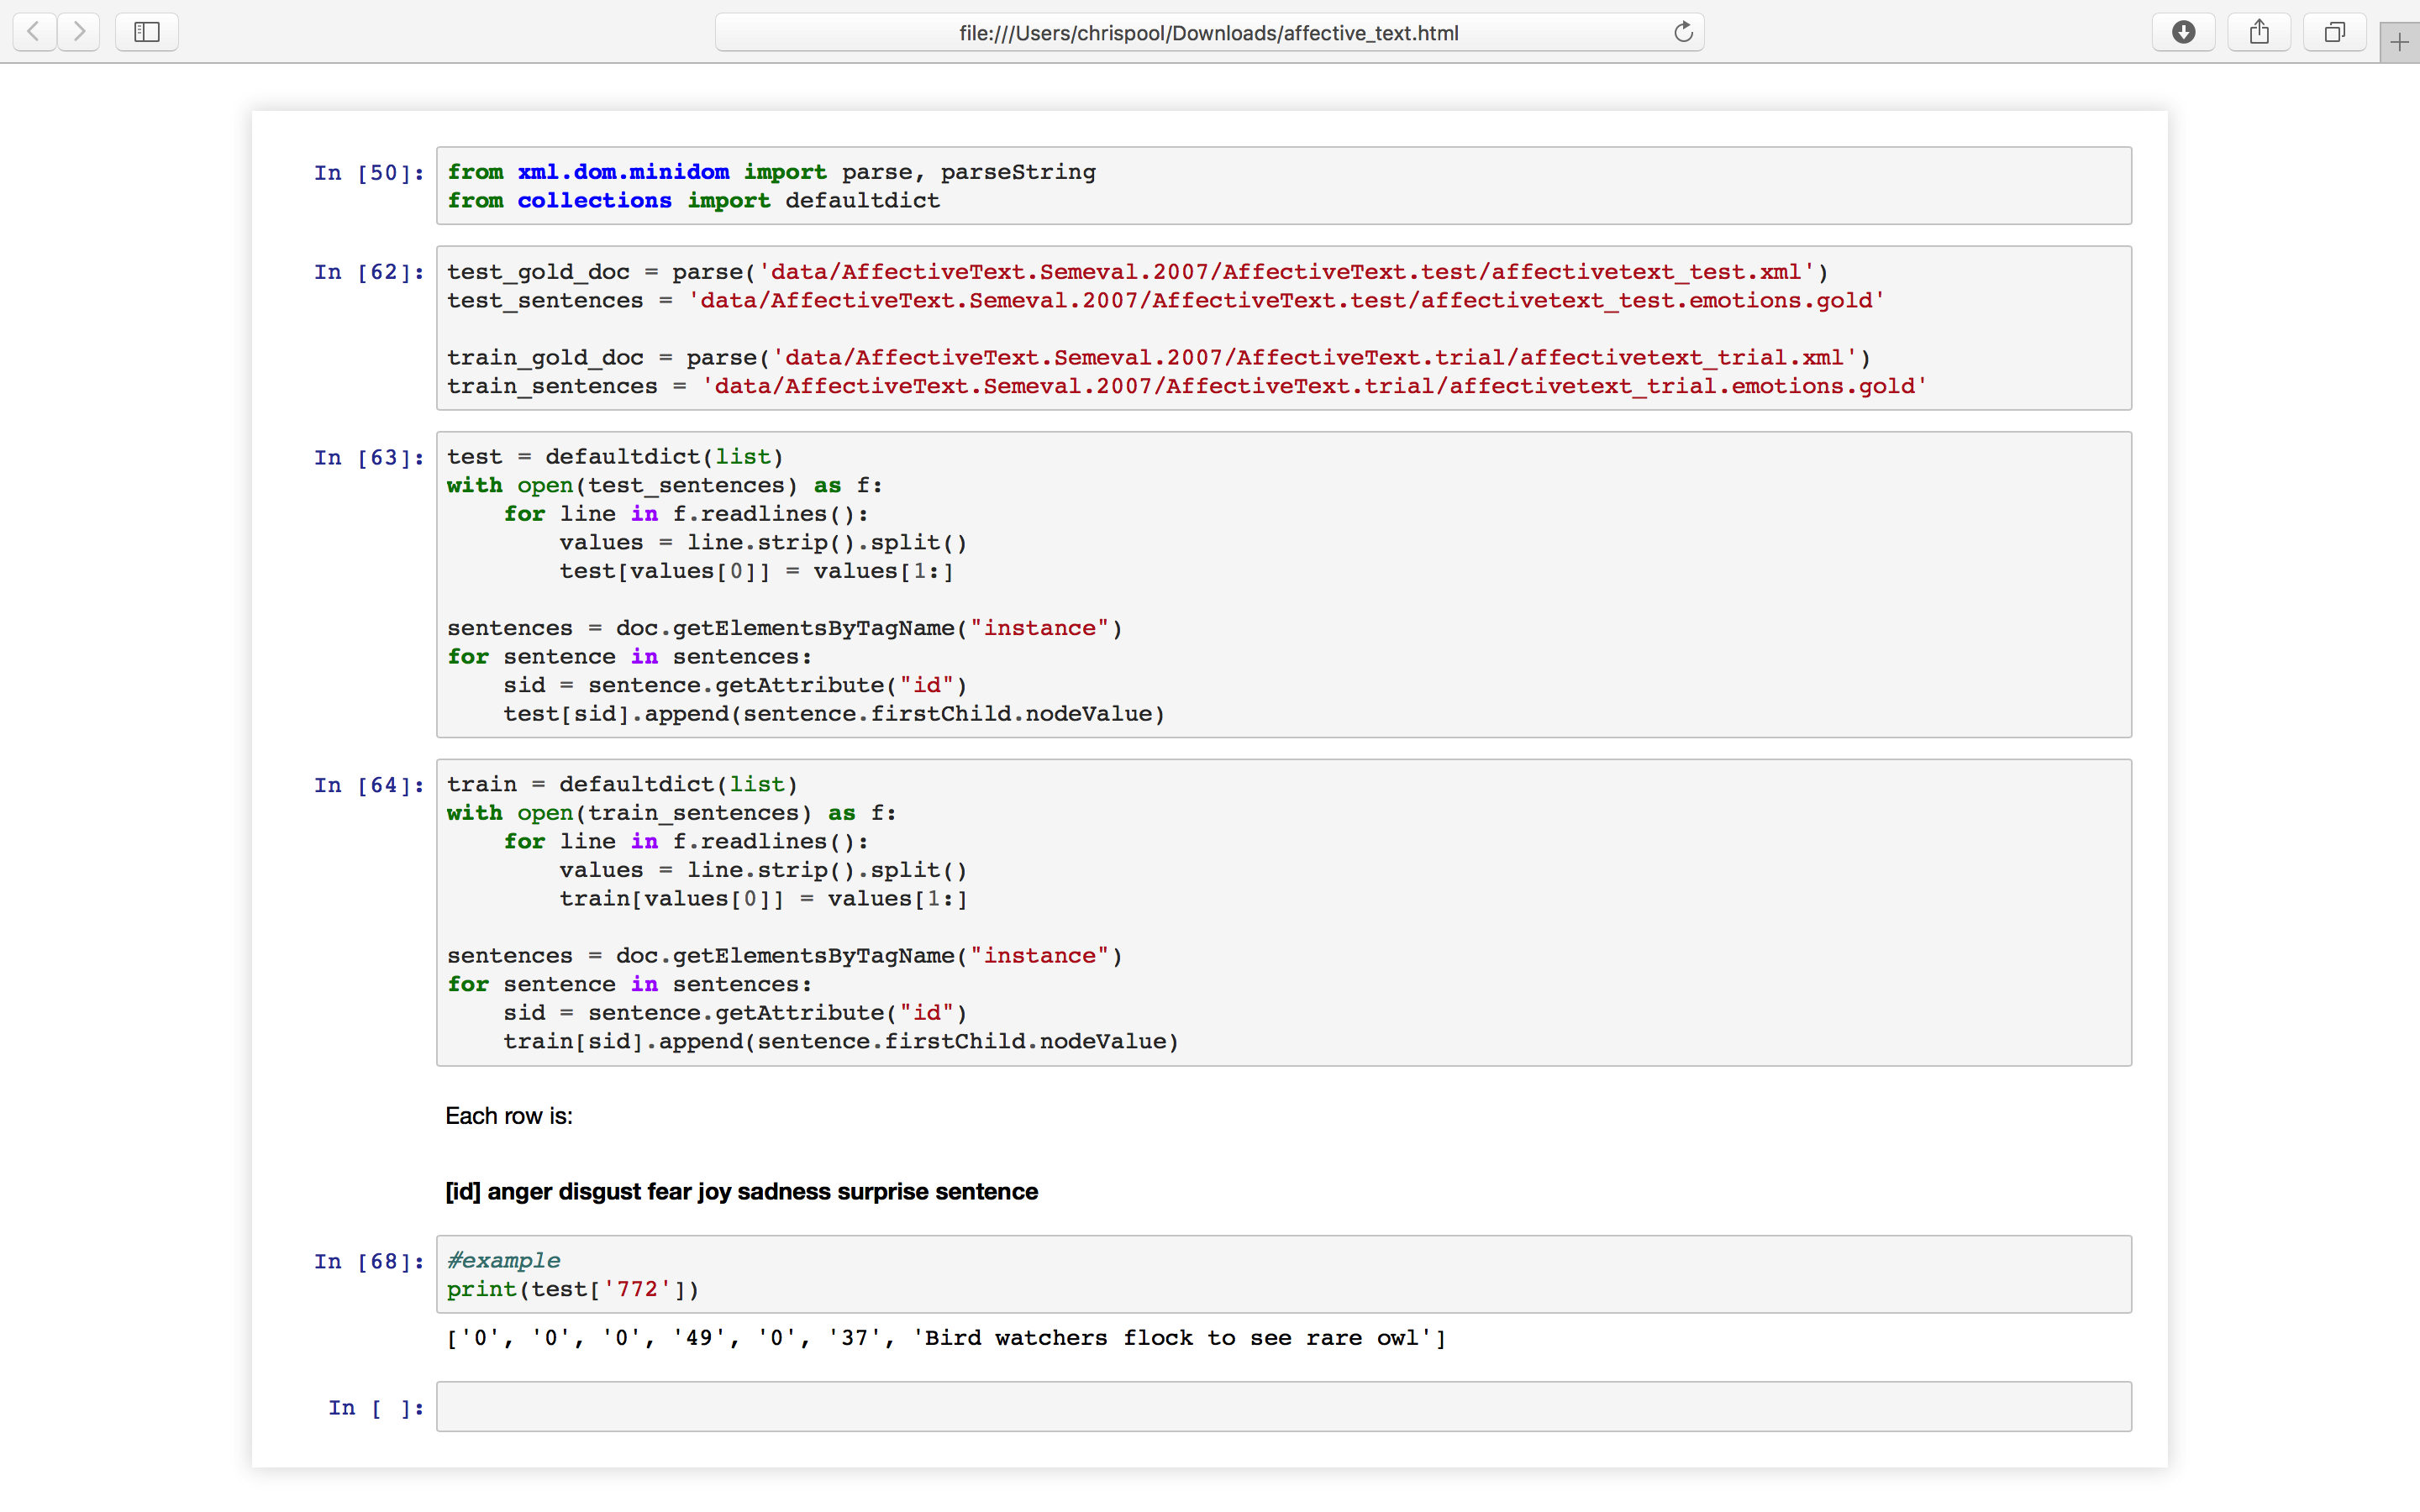
\includegraphics[width=\linewidth]{dataset_affective.png}
  \caption{Parsing the data-set using Jupyter Notebook (affective\_text.py)}
  \label{fig:dataset_affective}
\end{figure}
Figure \ref{fig:dataset_affective} is an example how to parse the data. The emotion vector indicates a strong Joy and Surprise emotion for the sentence \texttt{`Bird watchers flock to see rare owl`}.


\subsection{Fairy tales dataset}
This data was collected by \newcite{alm2008affect} as part of her PhD Dissertation\cite{alm2008affect}. This research is an exploration in detecting affect in text. For the research a data-set was created where fairy tales where annotated by two persons with an emotion (\texttt{Angry, Disgusted, Fearful, Happy, Sad} and \texttt{ surprised}). Fairy tales  from B. Potter, H.C. Andersen and Grimm's are used. In most researches that use this data-set (\cite{kim2010evaluation}, \cite{calvo2013emotions} and \cite{chaffar2011using}) only sentences with high agreement are used (four identical labels). The Affective Labels are in most researches: Angry-Disgusted, Fearful, Happy, Sad, and Surprised. I followed this mapping.

% Description of the dataset
The data-set contains four folders containing the raw data where for each sentence there are four annotations. A data-set that only contain the sentences with a high agreement are stored in a different folder and is used for most researches. The definition of high agreement is in this case where all the four labels are the same.

 
% Overview in which papers this data set was used
\newcite{chaffar2011using} used the Fairy tales data-set to evaluate a supervised model using features like bag-of-words, N-grams and lexical emotion features. The paper fails to mention which emotion categories were used. The results are based on cross-validation and were reported using accuracy scores and can be found in section 5.

In the paper by \cite{kim2010evaluation} they evaluated several unsupervised techniques using, among others, this data-set as described previously. Only the sentences with a high agreement (all four labels the same) were used. The results from this research are discussed in section 5. 

\begin{figure}[htb]
  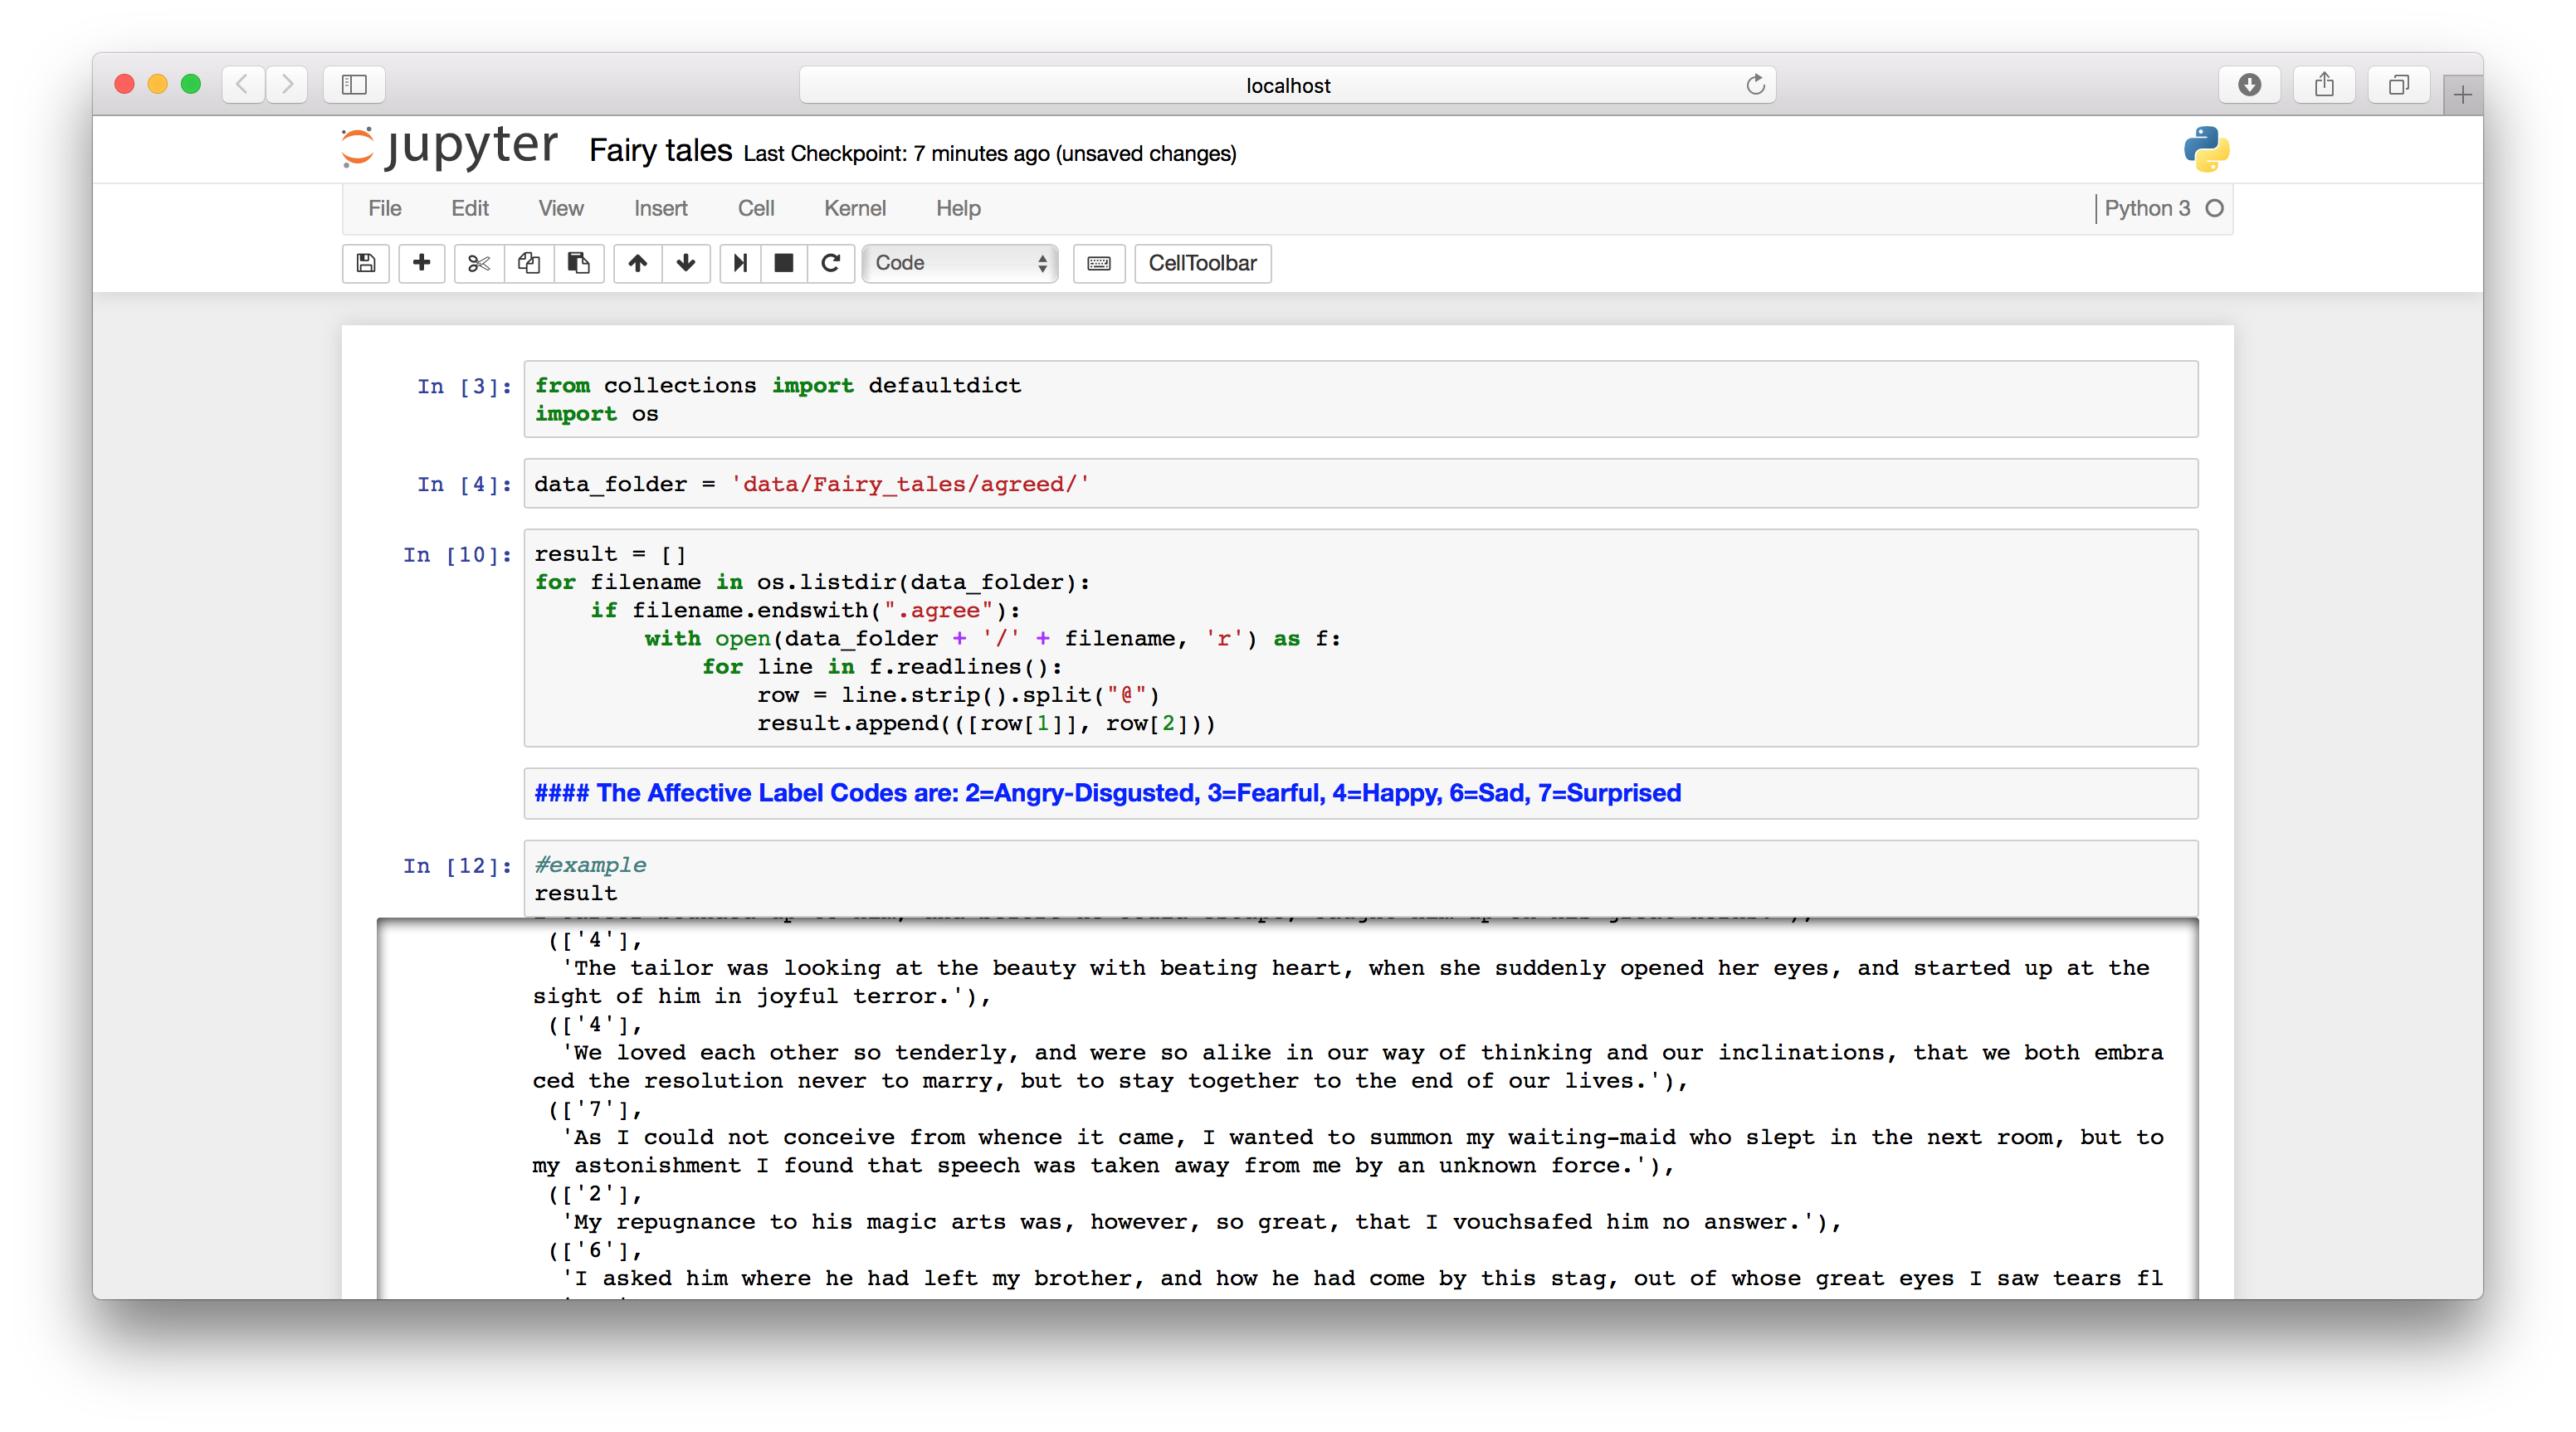
\includegraphics[width=\linewidth]{dataset_fairy-tales.png}
  \caption{Parsing the dataset using Jupyter Notebook (fairy-tales.py}
  \label{fig:dataset_fairy-tales}
\end{figure}

Figure \ref{fig:dataset_fairy-tales} is an example how to parse the data. Each item in the list is a tuple of the emotion and the sentence, an example can be found below.
\begin{lstlisting}[language=python, caption=Fairy tales example]
('4', 'We loved each other so tenderly, and were so alike 
in our way of thinking and our inclinations, that we both 
embraced the resolution never to marry, but to stay together 
to the end of our lives.')
\end{lstlisting}
In the documentation can be found that the \texttt{4} indicates a Joy full emotion.


\subsection{ISEAR}
The ISEAR (International Survey on Emotion Antecedents and Reactions) is a data-set that contains 7,665 sentences. The data-set is created by using questionnaires from participants with different cultural backgrounds. The questionnaires contained questions about experiences and reactions for seven emotions including: \texttt{anger, disgust, fear, joy, sadness, shame and guilt}. 


During the 1990s, a group of psychologists gathered data for the ISEAR project. Student respondents, both psychologists and non-psychologists, were asked to report situations in which they had experienced all of 7 major emotions (\texttt{joy, fear, anger, sadness, disgust, shame} and \texttt {guilt}). In each case, the questions covered the way they had appraised the situation and how they reacted. The final data-set contained reports on seven emotions each by close to 3000 respondents in 37 countries on all 5 continents.

% Overview in which papers this data set was used
In the paper by \newcite{kim2010evaluation} and \newcite{calvo2013emotions} they evaluated several unsupervised techniques using, among others, this data-set. The results from this paper are discussed in section 5 \cite{kim2010evaluation} and \cite{calvo2013emotions }

The data is stored in a Microsoft Access database where each row contains, among other information, the emotion and the sentence. In total there are 7665 sentences labeled with an emotion.


\subsection{Overview}
The distribution for each data-set is different as can be seen in figure \ref{fig:distribution_data-sets}. 
\begin{figure}[hbt]
  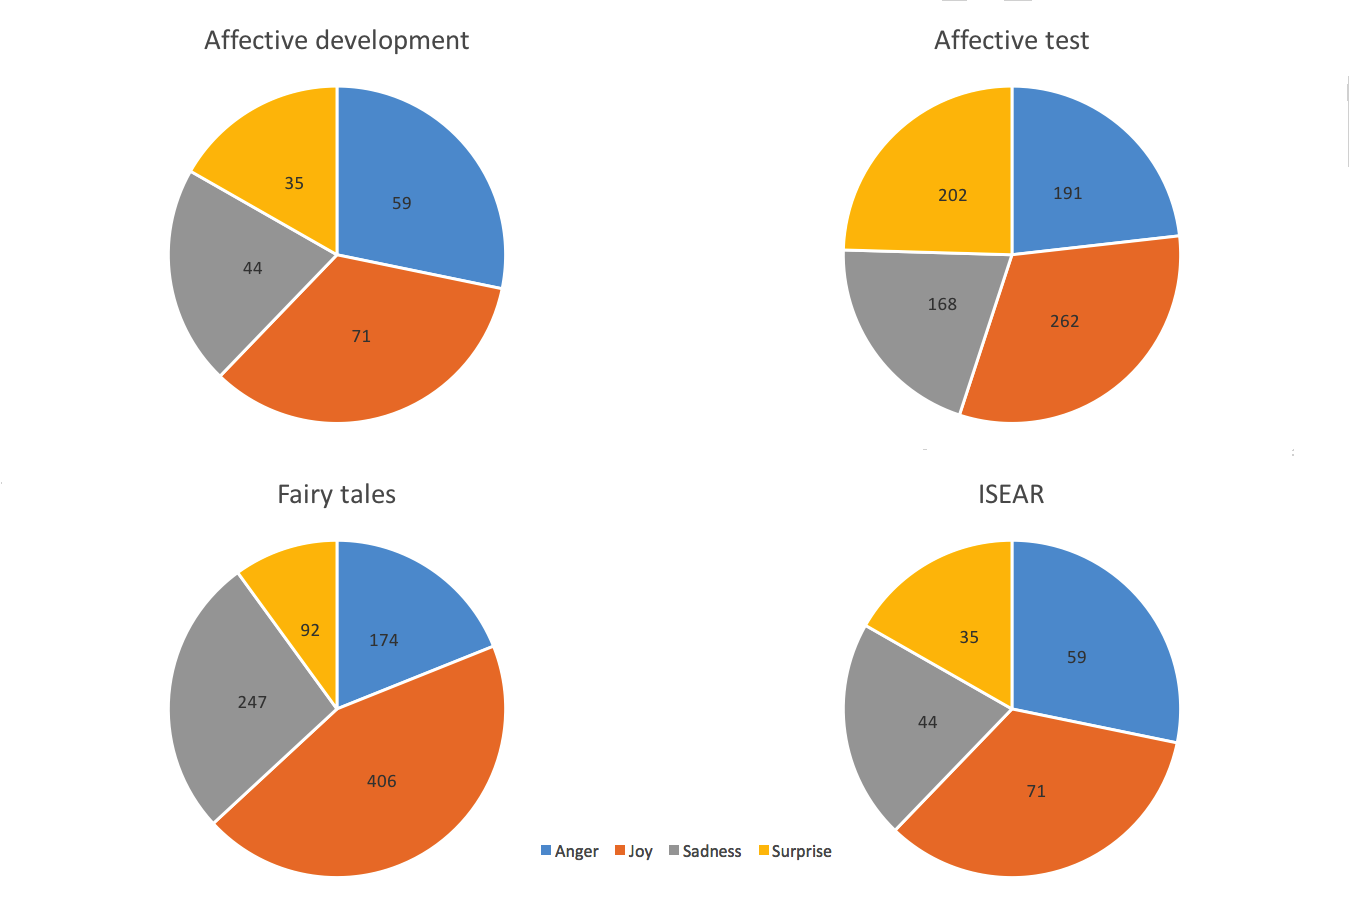
\includegraphics[width=\linewidth]{distribution_data.png}
  \caption{Distribution data-sets}
  \label{fig:distribution_data-sets}
\end{figure}
In table \ref{overview_data-sets} an overview can be found of emotions used in the data-sets described in the previous sections. For developing my system the intersection of emotions are used and are mentioned in the \texttt{Mapped} column.
\begin{table}[htb]
\centering

\begin{tabular}{|l|l|l|l|l|}
\hline
\textbf{SemEval} & \textbf{Fairy tales} & \textbf{ISEAR} & \textbf{Facebook} & \textbf{Mapped} \\ \hline
Anger            & Angry-Disgusted      & Anger               & Angry   & ANGER          \\ \hline
Disgust          & Angry-Disgusted      & Disgust               &    &  ANGER              \\ \hline
Fear             & Fearful              & Fear               &      &              \\ \hline
Joy              & Happy                & Joy                & Haha, Love & JOY\\ \hline
Sadness          & Sad                  & Sadness               & Sad     & SADNESS          \\ \hline
Surprise         & Suprised             &                & Wow          & SURPRISE     \\ 
\hline
                 &                      & Shame               &       &         \\ \hline
                 &                      & Guilt               &       &         \\                  
\hline
\end{tabular}
\caption{Mapping emotions}
\label{overview_data-sets}
\end{table}


\section{Experiment}
As experiment I trained a model using the Facebook data set that was obtained using the API as described in section 3. I evaluated my system by testing on other data-sets that are used in several other researches. I also experimented what the effect is of using different sets of Facebook pages. The idea is that by selecting pages similar to the test set (same domain) the results will improve.

\subsection{Getting the data}
The data on Facebook can be retrieved using the Facebook API. With the Facebook library for Python, written by Martey Dodoo \footnote{https://pypi.python.org/pypi/facebook-sdk}, it was fairly easy to retrieve posts and the corresponding reactions from several public pages on Facebook. Facebook Reactions is a new way for users to respond to posts. It enables users respond not only with a \texttt{like} but also with more detailed emotions (i.e. \texttt{Angry, Happy, Sad, Wow and Haha}). I choose to use the latest 1000 posts from each page because the reaction feature is fairly new and older posts don't contain this information. \\\\
By parsing the JSON files that are described in section three, in Python a list is created with the structure as described below:
\begin{lstlisting}[language=python]
train_data = [
  ['SADNESS', 'Sweden was once one of the most welcoming countries
  for refugees. Now that\'s changing.'],
  ['JOY', 'Thank goodness wine made the list.'],
  [...]
]
\end{lstlisting}

\subsection{Evaluation}
For evaluation I will use a small portion of the Affective data set described in section four. This data-set consists of two separate sets: a train set and a test set. During development I will use this train set that will be referred to as the \textit{development set} in this section, all results in this section are based on this set. In the final evaluation I will not use this data set. The development set contains 250 annotated sentences.

\subsection{Selecting Facebook Pages}
\begin{figure}[htb]
  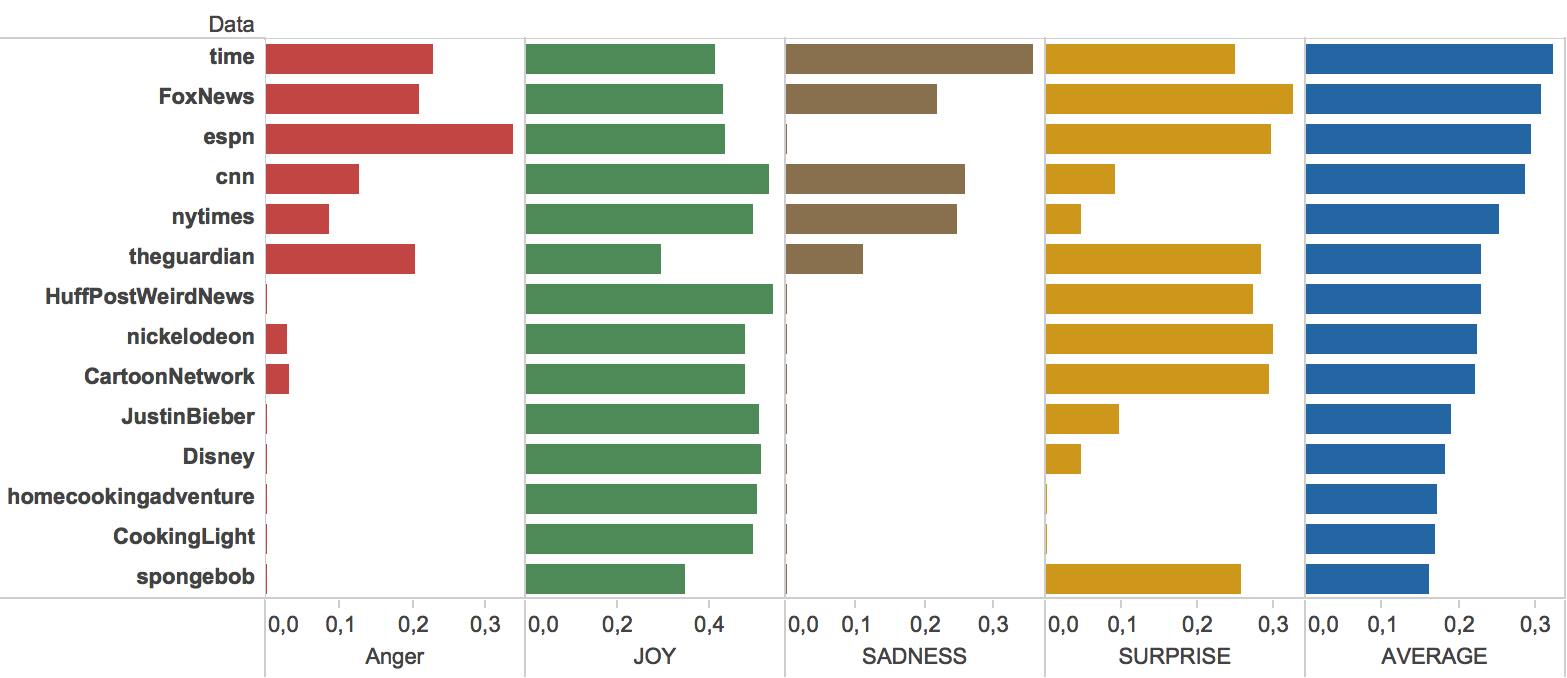
\includegraphics[width=\linewidth]{dataset.png}
  \caption{F-score per Facebook page}
  \label{fig:dataset_facebook}
\end{figure}
Figure \ref{fig:dataset_facebook} shows the results of classification using a single Facebook page to train on and tested on the development set using Support Vector Machine(SVM) and using the bag-of-words feature. The figure shows that there is a correlation between number of posts per emotions and the performance of that emotion, making a combined training set using several Facebook pages a good approach. To test the influence of using different Facebook pages I tested three models: \\
\begin{enumerate}
\item Model created using three Facebook pages that have the highest performance on the development set
\item Model created using three Facebook pages that following intuition will perform the best on the fairy tales data set.
\item Model created using three Facebook pages that following intuition will perform the best on the ISEAR data set.
\end{enumerate}

\subsubsection{Best performing model}
For the first model I looked at the best performing model on the development set using a combination of three Facebook pages. All results can be found in \ref{fig:datasets_facebook}. The combined set of the Facebook pages \texttt{Time, The Guardian} and \texttt{Disney} yields the highest results. \texttt{Time} and \texttt{The Guardian} perform good on most emotions but \texttt{Disney} helps to boost the performance for the \texttt{Joy} class.

\begin{figure}[htb]
  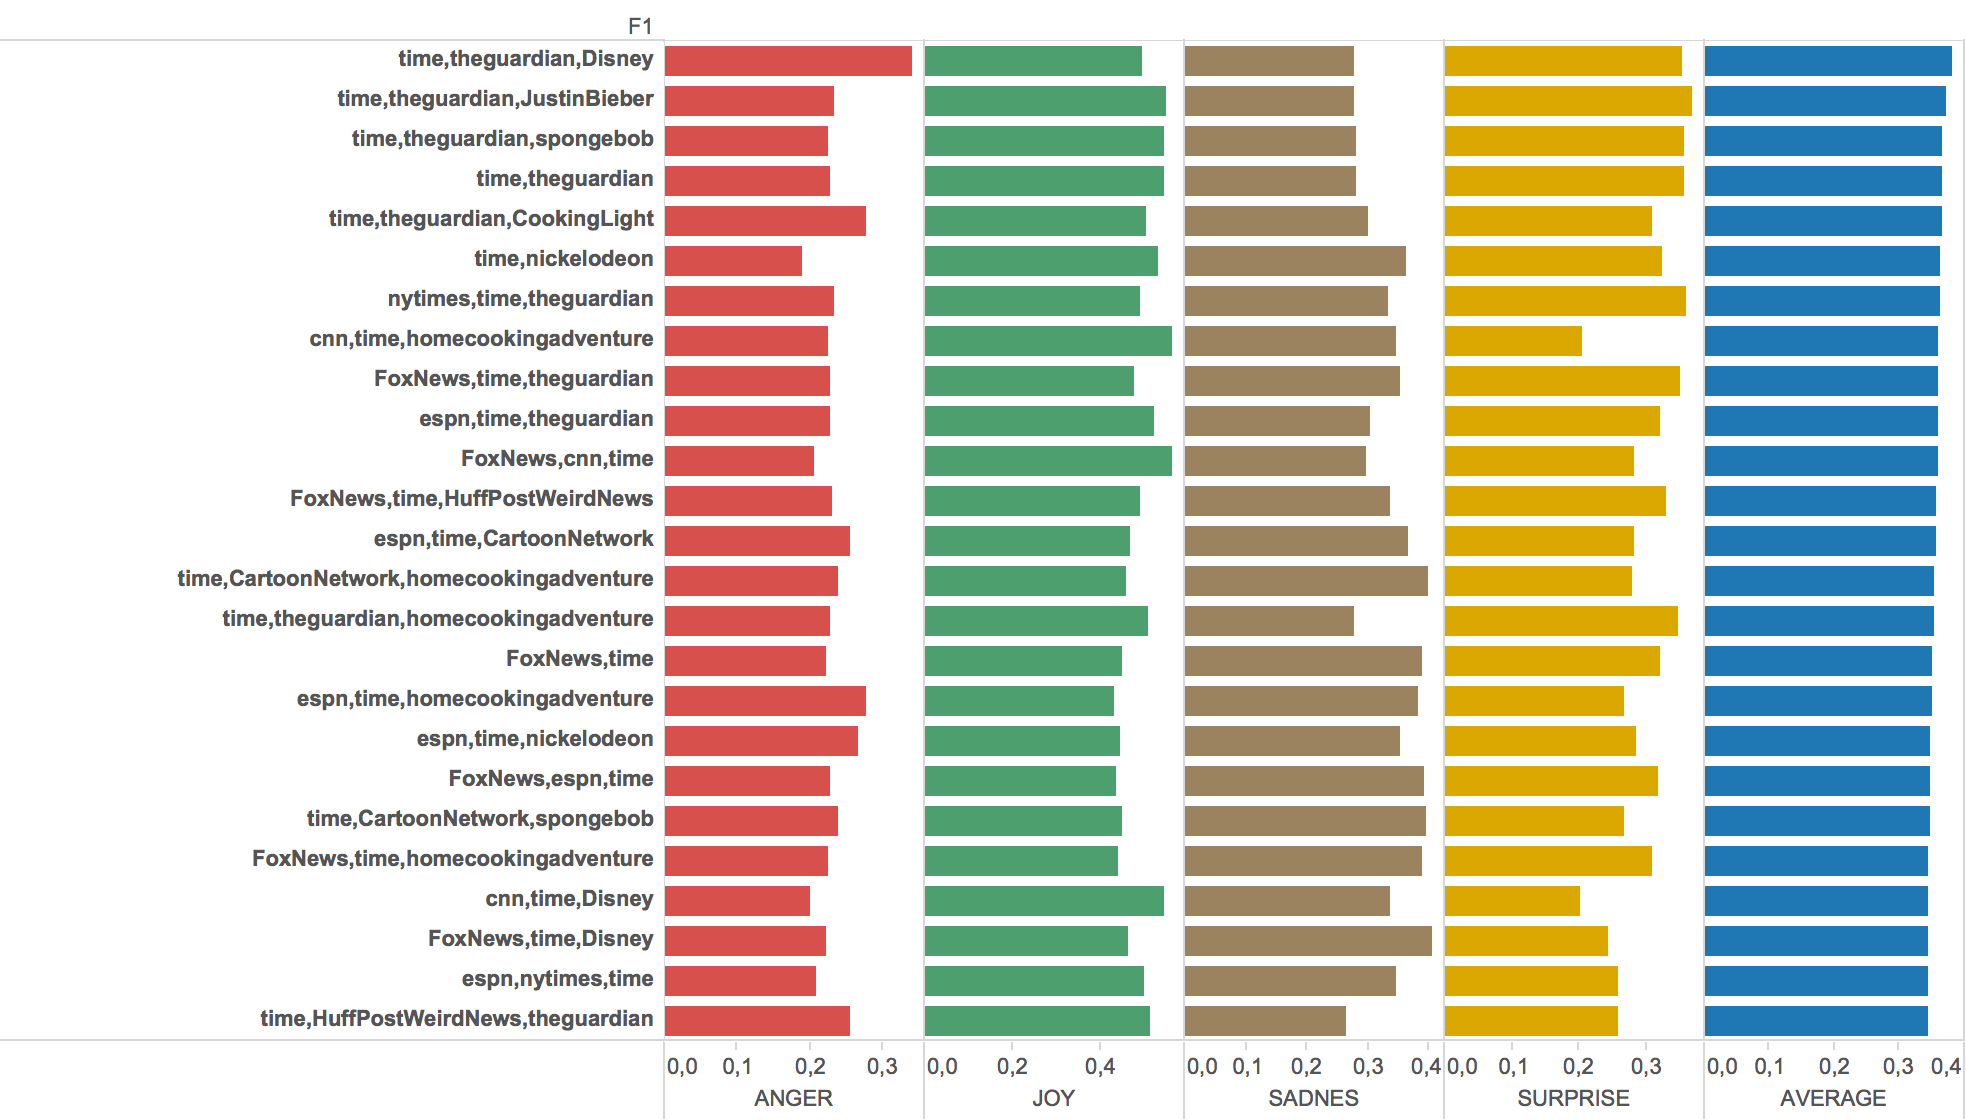
\includegraphics[width=\linewidth]{3datasets.png}
  \caption{F-score per Facebook page (combination of pages)}
  \label{fig:datasets_facebook}
\end{figure}

\subsubsection{Model for Fairy Tales data-set}
The sentences in the Fairy Tales data-set are quite different compared to the news headlines in the development set. Looking at the distribution in this data-set, as can be seen in figure \ref{fig:distribution_data-sets}, the \texttt{Joy} class is most frequent. I selected the pages \texttt{HuffPostWeirdNews, ESPN} and \texttt{CNN} for this model following intuition and looking at the performance for the emotions that are most frequent in the fairy tales data-set.

\subsubsection{Model for ISEAR data-set}
As described in section four the sentences in the ISEAR data-set are different compared to the two other data-sets. Looking at the distribution in this data-set as can be seen in \ref{fig:distribution_data-sets} and following intuition I selected the pages \texttt{Time, The Guardian} and \texttt{CookingLight} for this model. Because there is no \texttt{Surprise} emotion in the ISEAR data-set the importance to have training data for that category is none.

\subsection{Features}
In choosing features to detect emotions in text, I relied on previous work and on my intuition. Because the training data is from a different domain then the target domain the challenge is to create general models that are not domain specific. The evaluation of used features is done on the Affective text data-set. The final evaluation is done on other data from other domains. The contribution of the features to our models performance can be found in table \ref{test_results_svm}.

\subsubsection{Bag of words}
This basic features uses words as feature. I used the TF-idf, which is a measure to assign a weight to important words. Words that appear in each document are less relevant since it doesn\'t help in classification.

\subsubsection{N-grams}
N-gram-based features have proven to be a good performing feature in various researches about emotion detection. At the token level, features with uni-grams, bi-grams and tri-grams were implemented. The character-level features consisted of n-grams of 2 to 5 characters. 

\subsubsection{Affect Lexicons}
\newcite{mohammad:2012:NAACL-HLT} explores the performance of the different lexicons: NRC10 \cite{Mohammad13} and WordNet Affect\cite{strapparava2004wordnet}. I used the NRC10 lexicon as lexicon because it performed the best in the experiments by \cite{mohammad:2012:NAACL-HLT}. \\
For each word in the lexicon there is a Boolean value whether it contains that emotion or not. For example the word \texttt{FUN}:
\begin{lstlisting}[language=python]
fields = ['anger', 'anticipation', 'disgust', 'fear', 'joy',
'negative', 'positive', 'sadness', 'surprise', 'trust']
fun  = [0,1,0,0,1,0,1,0,0,0]

[field for field, fun in zip(fields, fun) if fun == 1]
--> 'anticipation', 'joy', 'positive'
\end{lstlisting}
For each sentence the sum of this vector is calculated and used as feature as can be seen in table \ref{feature_lexicon}.

\begin{table}[hbt]
\centering


\begin{tabular}{ll}

victims                            & {[}1, 0, 0, 1, 0, 1, 0, 1, 0, 0{]}                               \\
terror                             & {[}0, 0, 0, 1, 0, 1, 0, 0, 0, 0{]}                               \\
attack                             & {[}1, 0, 0, 1, 0, 1, 0, 0, 0, 0{]}                               \\
remembered                         & {[}0, 0, 0, 0, 0, 0, 0, 0, 0, 0{]}                               \\
tribute                            & {[}0, 0, 0, 0, 0, 0, 1, 0, 0, 0{]}                               \\
National                           & {[}0, 0, 0, 0, 0, 0, 0, 0, 0, 0{]}                               \\
Memorial                           & {[}0, 0, 0, 0, 0, 0, 0, 0, 0, 0{]}                               \\ \hline
\textbf{SUM} & {[}2, 0, 0, 3, 0, 3, 1, 1, 0, 0{]} \\ 
\end{tabular}
\caption{Score for \texttt{'victims of the terror attack in Orlando are remembered in a tribute at the National September 11 Memorial \& Museum.'}}
\label{feature_lexicon}
\end{table}


\subsubsection{Negations}
Negation is the grammatical operation whereby a proposition is replaced by one that states the opposite. An affirmative form expresses the validity or truth of a basic assertion. A negative form expresses the falsity of a basic assertion. In the English language, sentences may be negated with the adverbs \textit{not} and \textit{never}, the determiner \textit{no}, and the indefinite pronouns \textit{no one}, \textit{nobody}, and \textit{none} as well as other negative words.

\subsection{Training}
For training a model I used Scikit-learn \cite{scikit-learn}. 
\begin{lstlisting}[language=python, caption=Training a emotion classifier, label=trainmodel_py]

def classify_and_evaluate(train, test):
    X = [x for y, x, s in train if y != 'NONE']
    y = [y for y, x, s in train if y != 'NONE']

    pipeline = Pipeline([
        ('features', FeatureUnion([
            ('lexicon_nrc', features.NRCLexicon()),
            ('words', TfidfVectorizer(stop_words='english')),
            ('token_ngrams', TfidfVectorizer(stop_words='english', ngram_range = (2, 5))),
            ('char_ngrams', TfidfVectorizer(ngram_range = (2, 5), analyzer = 'char')),
            ('negation', features.Negation() ),  
            ('punctuation', features.Punctuation() ),  
        ])),
        ('classifier', svm.SVC(kernel='linear', C=0.5, class_weight = 'balanced'))
    ])
    pipeline.fit(X, y)
    X_test = [x for y, x in test if y != 'NONE']
    y_test = [y for y, x in test if y != 'NONE']
    y_pred = pipeline.predict(X_test)
    print(classification_report(y_test, y_pred))
    print(confusion_matrix(y_test, y_pred))
\end{lstlisting}
The code in example five shows that it is fairly easy in Scikit-learn to create a pipeline for Machine Learning. This function uses the train data to train a model and uses the test data to evaluate the model. All results are obtained using this pipeline.

\subsection{Results on development set}
As described, all evaluation is done on the development set. Most researches report their results in Precision, recall and F-score. I therefore also used these metrics. 

\begin{table}[!htbp]
\centering
\begin{tabular}{|l|l|l|l|l|l|}
\hline
    Feature & ANGER & JOY & SAD. & SURP. & \textbf{AVG.} \\ 

\hline
  \footnotesize{TF-idf} &
  \footnotesize{0.57,0.22,0.32}  & 
  \footnotesize{0.44,0.51,0.47} & 
  \footnotesize{0.41,0.25, 0.31} & 
  \footnotesize{0.22,0.49,0.30} & 
  \footnotesize{\textbf{0.43,0.37,0.37}}  \\ 

\hline
  \footnotesize{Lexicon} &
  \footnotesize{0.28,0.08,0.13}  & 
  \footnotesize{0.43,0.37,0.40} & 
  \footnotesize{0.31,0.30, 0.30} & 
  \footnotesize{0.20,0.51,0.29} & 
  \footnotesize{\textbf{0.32,0.30,0.28}}  \\ 

\hline
  \footnotesize{Negation} &
  \footnotesize{0.35,0.10,0.16}  & 
  \footnotesize{0.35,0.94,0.51} & 
  \footnotesize{0.00,0.00, 0.00} & 
  \footnotesize{0.00,0.00,0.00} & 
  \footnotesize{\textbf{0.22,0.35,0.22}}  \\ 

\hline
  \footnotesize{Token n-grams(2,5)} &
  \footnotesize{0.00,0.00,0.00}  & 
  \footnotesize{1.00,0.01,0.03} & 
  \footnotesize{0.00,0.00, 0.00} & 
  \footnotesize{0.17,1.00,0.29} & 
  \footnotesize{\textbf{0.37,0.17,0.06}}  \\ 

\hline
  \footnotesize{Character n-grams(2,5)} &
  \footnotesize{0.50,0.03,0.06}  & 
  \footnotesize{0.39,0.73,0.51} & 
  \footnotesize{0.38,0.07, 0.12} & 
  \footnotesize{0.17,0.31,0.22} & 
  \footnotesize{\textbf{0.38,0.33,0.25}}  \\ 

\hline
  \footnotesize{Punctuation} &
  \footnotesize{0.28,0.97,0.44}  & 
  \footnotesize{0.50,0.01,0.03} & 
  \footnotesize{0.50,0.05, 0.08} & 
  \footnotesize{0.00,0.00,0.00} & 
  \footnotesize{\textbf{0.35,0.29,0.15}}  \\ 

\hline
  \footnotesize{All features} &
  \footnotesize{0.40,0.03,0.06}  & 
  \footnotesize{0.35,0.97,0.52} & 
  \footnotesize{0.62,0.11, 0.19} & 
  \footnotesize{1.00,0.03,0.06} & 
  \footnotesize{\textbf{0.35,0.29,0.15}}  \\ 

\hline
  \footnotesize{TF-idf \& Lexicon} &
  \footnotesize{0.61,0.24,0.34}  & 
  \footnotesize{0.44,0.56,0.49} & 
  \footnotesize{0.36,0.23, 0.38} & 
  \footnotesize{0.27,0.51,0.35} & 
  \footnotesize{\textbf{0.44,0.39,0.38}}  \\ 

\hline
  \footnotesize{TF-idf \&Lexicon \& Punctuation} &
  \footnotesize{0.52,0.29,0.37}  & 
  \footnotesize{0.45,0.72,0.55} & 
  \footnotesize{0.48,0.23, 0.31} & 
  \footnotesize{0.24,0.29,0.26} & 
  \footnotesize{\textbf{0.44,0.42,0.40}}  \\ 




\hline                
\end{tabular}
\caption{Results on test set using Support Vector Machine}
\label{test_results_svm}
\end{table}
\subsection{Test results}
The final test results can be found in table \ref{final_results}. For comparison I looked at some researches that use the same data-set that are described in section four.

\subsubsection{\newcite{kim2010evaluation}}
In this paper \cite{kim2010evaluation} they experimented with 4 different approaches, all unsupervised techniques. The results were reported using the precision, recall and F-score metric for each emotion category and can be found for the CNMF-based categorical classification (best average performing approach). There are no results for \texttt{Surprise} because they ignored this emotion since it is not present in the ISEAR data-set.

\subsubsection{\newcite{strapparava2008learning}}
\cite{strapparava2008learning} experimented with several models, the \texttt{LSA - all emotion words} yielded the highest average results, therefore only these results are mentioned in table \ref{final_results}.

\subsubsection{\newcite{danisman2008feeler}}
In this research \cite{danisman2008feeler} they describe training a model using the ISEAR data-set and test on the Affective text data-set. Reports for each category are only reported in terms of F-score.

\subsubsection{Best model}
The \textit{best model} uses the Facebook pages \texttt{time, theguardian} and \texttt{Disney}. This is based on the performance on the development set. Expected is that this model also performs the best on the Affective test-set since it is the same domain. The results that can be found in table \ref{test_results_svm} show that it indeed performed the best on the Affective data-set together with \textit{Model 1}, although the difference among the models is not that big. The performance on the other data-sets is almost similar to  \textit{Model 1} and \textit{Model 2}\\\\
Interesting is that the model seems to have difficulties to distinguish the \texttt{Joy} and \texttt{Surprise} class. For all classes the model has a high bias for the \texttt{Joy} class. The model evaluated using the ISEAR data-set also seems to have difficulties with especially the \texttt{Anger} and \texttt{Surprise} class.
\begin{table}[hbt]
            \footnotesize
                \begin{tabular}[t]{|l|c|c|c|c|}
                    \hline
                    \multicolumn{5}{|c|}{{Affective}} \\    
                    \hline
                    &a&b&c&d\\ \hline
                    a&37&87&21&46 \\ \hline
                    b&20&168&4&70\\ \hline
                    c&28&75&35&30 \\ \hline   
                    d&23&117&9&53\\ \hline
                \end{tabular}
                \hfill
                \begin{tabular}[t]{|l|c|c|c|c|}
                    \hline
                    \multicolumn{5}{|c|}{{Fairy tales}} \\    
                    \hline
                    &a&b&c&d\\ \hline
                    a&33&54&30&57 \\ \hline
                    b&13&278&34&81\\ \hline
                    c&37&88&62&60 \\ \hline   
                    d&4&58&9&21\\ \hline
                \end{tabular}
                \hfill
                \begin{tabular}[t]{|l|c|c|c|c|}
                    \hline
                    \multicolumn{5}{|c|}{{ISEAR}} \\    
                    \hline
                    &a&b&c&d\\ \hline
                    a&157&298&322&318 \\ \hline
                    b&53&584&102&353\\ \hline
                    c&93&341&421&240 \\ \hline   
                    d&0&0&0&0\\ \hline
                \end{tabular}
                \caption{Confusion Matrices for the Best model}
                \label{Confusion Matrices for the Best model}
                *a = Anger, b = Joy, c= Sadness, d = Surprise
            \end{table}

\subsubsection{Model 1}
The \textit{Model 1} uses the Facebook pages \texttt{HuffPostWeirdNews, ESPN} and \texttt{CNN}. This is based on intuition and looking at the target domain. Expected is that this model performs the best on the Fairy tales test-set since it is the same domain. The results that can be found in table \ref{test_results_svm} show that it indeed performed the best on the Fairy tales data-set together with the \textit{Best performing model} although the difference among the models is not that big. The performance on the other data-sets is almost similar to  \textit{Best performing model} and \textit{Model 2}\\\\
Model 1 has the same problem as \textit{Best model}, it has a high bias towards \texttt{Joy}. Looking at the confusion matrices in table\ref{Confusion Matrices for the model 1} the model seems to perform better for the \texttt{Surprise} class, but being a small class it does not improve overall performance that much.

\begin{table}[hbt]
            \footnotesize
                \begin{tabular}[t]{|l|c|c|c|c|}
                    \hline
                    \multicolumn{5}{|c|}{{Affective}} \\    
                    \hline
                    &a&b&c&d\\ \hline
                    a&30&62&11&88 \\ \hline
                    b&11&123&9&119\\ \hline
                    c&16&36&28&88 \\ \hline   
                    d&14&83&4&101\\ \hline
                \end{tabular}
                \hfill
                \begin{tabular}[t]{|l|c|c|c|c|}
                    \hline
                    \multicolumn{5}{|c|}{{Fairy tales}} \\    
                    \hline
                    &a&b&c&d\\ \hline
                    a&23&50&12&89 \\ \hline
                    b&20&252&22&112\\ \hline
                    c&21&63&63&100 \\ \hline   
                    d&3&34&5&50\\ \hline
                \end{tabular}
                \hfill
                \begin{tabular}[t]{|l|c|c|c|c|}
                    \hline
                    \multicolumn{5}{|c|}{{ISEAR}} \\    
                    \hline
                    &a&b&c&d\\ \hline
                    a&279&357&88&371 \\ \hline
                    b&56&604&55&377\\ \hline
                    c&99&375&313&308 \\ \hline   
                    d&0&0&0&0\\ \hline
                \end{tabular}
                \caption{Confusion Matrices for the model 1}
                \label{Confusion Matrices for the model 1}
                *a = Anger, b = Joy, c= Sadness, d = Surprise
            \end{table}

\subsubsection{Model 2}
The \textit{model 2} uses the Facebook pages \texttt{time, theguardian} and \texttt{CookingLight}. This is based intuition and looking at the target domain. Expected is that this model performs the best on the ISEAR test-set since it is the same domain. The results that can be found in table \ref{test_results_svm} show that it does not performed the best on the ISEAR data-set. \textit{Model 1}  performed the best although the difference among the models is not that big. The performance on the other data-sets is almost similar to  \textit{Model 1} and \textit{Model 2}\\\\
Model 2 is overall the worst performing model. This is mostly due to the fact that it has the highest bias to the \texttt{Joy} class. For this individual class it performs pretty good especially for the Affective text data-set.

\begin{table}[hbt]
            \footnotesize
                \begin{tabular}[t]{|l|c|c|c|c|}
                    \hline
                    \multicolumn{5}{|c|}{{Affective}} \\    
                    \hline
                    &a&b&c&d\\ \hline
                    a&32&113&19&27 \\ \hline
                    b&15&208&3&36\\ \hline
                    c&25&97&31&15 \\ \hline   
                    d&17&142&9&34\\ \hline
                \end{tabular}
                \hfill
                \begin{tabular}[t]{|l|c|c|c|c|}
                    \hline
                    \multicolumn{5}{|c|}{{Fairy tales}} \\    
                    \hline
                    &a&b&c&d\\ \hline
                    a&28&71&32&43 \\ \hline
                    b&14&290&35&67\\ \hline
                    c&35&105&59&48 \\ \hline   
                    d&5&60&9&18\\ \hline
                \end{tabular}
                \hfill
                \begin{tabular}[t]{|l|c|c|c|c|}
                    \hline
                    \multicolumn{5}{|c|}{{ISEAR}} \\    
                    \hline
                    &a&b&c&d\\ \hline
                    a&142&383&344&226 \\ \hline
                    b&57&648&109&278\\ \hline
                    c&98&394&406&197 \\ \hline   
                    d&0&0&0&0\\ \hline
                \end{tabular}
                \caption{Confusion Matrices for model 2}
                \label{Confusion Matrices for model 2}
                *a = Anger, b = Joy, c= Sadness, d = Surprise
            \end{table}


\begin{table}[!htbp]
\centering

\begin{tabular}{|l|l|l|l|l|l|l|l|l|l|}
\hline
    & 
    \multicolumn{3}{|c|}{{Affective text}} & 
    \multicolumn{3}{|c|}{{Fairy Tales}} & 
    \multicolumn{3}{|c|}{{ISEAR}}  \\
        
\hline
    & 
    \textbf{P} & 
    \textbf{R} & 
    \textbf{F} & 
    \textbf{P} & 
    \textbf{R} & 
    \textbf{F} & 
    \textbf{P} & 
    \textbf{R} & 
    \textbf{F} \\ 
     
\hline                      
    \multicolumn{10}{|c|}{{ ANGER}} \\                 
                                         
\hline
    \tiny{Best performing model} & 
    \footnotesize{0.34} & 
    \footnotesize{0.19} & 
    \footnotesize{0.25} & 
    \footnotesize{0.38} & 
    \footnotesize{0.19} & 
    \footnotesize{0.25} & 
    \footnotesize{0.52} & 
    \footnotesize{0.14} & 
    \footnotesize{0.22} \\ 

\hline
    \tiny{Model 1} & 
    \footnotesize{0.42} & 
    \footnotesize{0.16} & 
    \footnotesize{0.23} & 
    \footnotesize{0.34} & 
    \footnotesize{0.13} & 
    \footnotesize{0.19} & 
    \footnotesize{0.64} & 
    \footnotesize{0.25} & 
    \footnotesize{0.36} \\ 

\hline
    \tiny{Model 2} & 
    \footnotesize{0.36} & 
    \footnotesize{0.17} & 
    \footnotesize{0.23} & 
    \footnotesize{0.34} & 
    \footnotesize{0.16} & 
    \footnotesize{0.22} & 
    \footnotesize{0.48} & 
    \footnotesize{0.13} & 
    \footnotesize{0.21} \\ 


\hline
    \tiny{\cite{strapparava2008learning} } &
    \footnotesize{0.06} & 
    \footnotesize{0.88} & 
    \footnotesize{0.12} &
    &
    &
    &
    &
    &
    \\

\hline
    \tiny{\cite{kim2010evaluation} } &
    \footnotesize{0.29} & 
    \footnotesize{0.26} & 
    \footnotesize{0.28} &
    \footnotesize{0.77} & 
    \footnotesize{0.56} & 
    \footnotesize{0.65} &
    \footnotesize{0.41} & 
    \footnotesize{0.99} & 
    \footnotesize{0.58} \\
    
\hline
    \tiny{\cite{danisman2008feeler} } &
    \footnotesize{} & 
    \footnotesize{} & 
    \footnotesize{0.24} &
    \footnotesize{} & 
    \footnotesize{} & 
    \footnotesize{} &
    \footnotesize{} & 
    \footnotesize{} & 
    \footnotesize{} \\


\hline
    \multicolumn{10}{|c|}{{FEAR}} \\ 

\hline
    \tiny{Best Performing model} & 
    \footnotesize{0.00} & 
    \footnotesize{0.00} & 
    \footnotesize{0.00} & 
    \footnotesize{0.00} & 
    \footnotesize{0.00} & 
    \footnotesize{0.00} & 
    \footnotesize{0.00} & 
    \footnotesize{0.00} & 
    \footnotesize{0.00} \\ 

\hline
    \tiny{Model 1} & 
    \footnotesize{0.00} & 
    \footnotesize{0.00} & 
    \footnotesize{0.00} & 
    \footnotesize{0.00} & 
    \footnotesize{0.00} & 
    \footnotesize{0.00} & 
    \footnotesize{0.00} & 
    \footnotesize{0.00} & 
    \footnotesize{0.00} \\ 

\hline
    \tiny{Model 2} & 
    \footnotesize{0.00} & 
    \footnotesize{0.00} & 
    \footnotesize{0.00} & 
    \footnotesize{0.00} & 
    \footnotesize{0.00} & 
    \footnotesize{0.00} & 
    \footnotesize{0.00} & 
    \footnotesize{0.00} & 
    \footnotesize{0.00} \\     

\hline
    \tiny{\cite{strapparava2008learning} } &
    \footnotesize{0.13} & 
    \footnotesize{0.86} & 
    \footnotesize{0.22} & 
    &
    &
    &
    &
    &
    \\

\hline
    \tiny{\cite{kim2010evaluation} } &
    \footnotesize{0.53} & 
    \footnotesize{0.75} & 
    \footnotesize{0.62} &
    \footnotesize{0.70} & 
    \footnotesize{0.78} & 
    \footnotesize{0.74} &
    \footnotesize{0.69} & 
    \footnotesize{0.03} & 
    \footnotesize{0.06} \\

\hline
    \tiny{\cite{danisman2008feeler} } &
    \footnotesize{0.00} & 
    \footnotesize{0.00} & 
    \footnotesize{0.41} &
    \footnotesize{0.00} & 
    \footnotesize{0.00} & 
    \footnotesize{0.00} &
    \footnotesize{0.00} & 
    \footnotesize{0.00} & 
    \footnotesize{0.00} \\

\hline
    \multicolumn{10}{|c|}{{JOY}} \\ 

\hline
    \tiny{Best performing model} & 
    \footnotesize{0.38} & 
    \footnotesize{0.64} & 
    \footnotesize{0.47} & 
    \footnotesize{0.58} & 
    \footnotesize{0.68} & 
    \footnotesize{0.63} & 
    \footnotesize{0.48} & 
    \footnotesize{0.53} & 
    \footnotesize{0.50} \\ 

\hline
    \tiny{Model 1} & 
    \footnotesize{0.40} & 
    \footnotesize{0.47} & 
    \footnotesize{0.43} & 
    \footnotesize{0.63} & 
    \footnotesize{0.62} & 
    \footnotesize{0.63} & 
    \footnotesize{0.45} & 
    \footnotesize{0.55} & 
    \footnotesize{0.50} \\ 

\hline
    \tiny{Model 2} & 
    \footnotesize{0.37} & 
    \footnotesize{0.79} & 
    \footnotesize{0.51} & 
    \footnotesize{0.55} & 
    \footnotesize{0.71} & 
    \footnotesize{0.62} & 
    \footnotesize{0.45} & 
    \footnotesize{0.59} & 
    \footnotesize{0.51} \\ 

\hline 
    \tiny{\cite{strapparava2008learning} } &
    \footnotesize{0.19} & 
    \footnotesize{0.90} & 
    \footnotesize{0.31} &
    &
    &
    &
    &
    &
    \\

\hline
    \tiny{\cite{kim2010evaluation}} &
    \footnotesize{0.77} & 
    \footnotesize{0.58} & 
    \footnotesize{0.65} &
    \footnotesize{0.80} & 
    \footnotesize{0.76} & 
    \footnotesize{0.78} &
    \footnotesize{0.39} & 
    \footnotesize{0.01} & 
    \footnotesize{0.01} \\
    
\hline
    \tiny{\cite{danisman2008feeler}} &
    \footnotesize{} & 
    \footnotesize{} & 
    \footnotesize{0.50} &
    \footnotesize{} & 
    \footnotesize{} & 
    \footnotesize{} &
    \footnotesize{} & 
    \footnotesize{} & 
    \footnotesize{} \\
    
\hline
    \multicolumn{10}{|c|}{{SADNESS}} \\ 
    
\hline
    \tiny{Best performing model} & 
    \footnotesize{00.51} & 
    \footnotesize{00.21} & 
    \footnotesize{00.30} & 
    \footnotesize{00.46} & 
    \footnotesize{00.25} & 
    \footnotesize{00.32} & 
    \footnotesize{00.50} & 
    \footnotesize{00.38} & 
    \footnotesize{00.43} \\ 

\hline
    \tiny{Model 1} & 
    \footnotesize{00.54} & 
    \footnotesize{00.17} & 
    \footnotesize{00.25} & 
    \footnotesize{00.62} & 
    \footnotesize{00.26} & 
    \footnotesize{00.36} & 
    \footnotesize{00.69} & 
    \footnotesize{00.28} & 
    \footnotesize{00.40} \\ 

\hline
    \tiny{Model 2} & 
    \footnotesize{00.50} & 
    \footnotesize{00.18} & 
    \footnotesize{00.27} & 
    \footnotesize{00.44} & 
    \footnotesize{00.24} & 
    \footnotesize{00.31} & 
    \footnotesize{00.47} & 
    \footnotesize{00.37} & 
    \footnotesize{00.42} \\ 

\hline
    \tiny{\cite{strapparava2008learning} } &
    \footnotesize{0.12} & 
    \footnotesize{0.87} & 
    \footnotesize{0.22} &
    &
    &
    &
    &
    &
    \\

\hline
    \tiny{\cite{kim2010evaluation} } &
    \footnotesize{0.50} & 
    \footnotesize{0.45} & 
    \footnotesize{0.48} &
    \footnotesize{0.71} & 
    \footnotesize{0.82} & 
    \footnotesize{0.77} &
    \footnotesize{0.37} & 
    \footnotesize{0.01} & 
    \footnotesize{0.25} \\

\hline
    \tiny{\cite{danisman2008feeler}} &
    \footnotesize{} & 
    \footnotesize{} & 
    \footnotesize{0.37} &
    \footnotesize{} & 
    \footnotesize{} & 
    \footnotesize{} &
    \footnotesize{} & 
    \footnotesize{} & 
    \footnotesize{} \\

\hline
    \multicolumn{10}{|c|}{{SURPRISE}} \\                               
    
\hline
  \tiny{Best performing model} & 
  \footnotesize{0.27} & 
  \footnotesize{0.26} & 
  \footnotesize{0.26} & 
  \footnotesize{0.10} & 
  \footnotesize{0.23} & 
  \footnotesize{0.14} & 
  \footnotesize{} & 
  \footnotesize{} & 
  \footnotesize{} \\ 

\hline
    \tiny{Model 1} & 
    \footnotesize{0.26} & 
    \footnotesize{0.50} & 
    \footnotesize{0.34} & 
    \footnotesize{0.14} & 
    \footnotesize{0.54} & 
    \footnotesize{0.23} & 
    \footnotesize{} & 
    \footnotesize{} & 
    \footnotesize{} \\ 

\hline
    \tiny{Model 2} & 
    \footnotesize{0.30} & 
    \footnotesize{0.17} & 
    \footnotesize{0.22} & 
    \footnotesize{0.10} & 
    \footnotesize{0.20} & 
    \footnotesize{0.13} & 
    \footnotesize{} & 
    \footnotesize{} & 
    \footnotesize{} \\ 


\hline
    \tiny{\cite{strapparava2008learning} } &
    \footnotesize{0.08} & 
    \footnotesize{0.95} & 
    \footnotesize{0.14} &
    &
    &
    &
    &
    &
    \\

\hline
    \tiny{\cite{kim2010evaluation} } &
    & 
    & 
    &
    &
    &
    &
    &
    &
    \\
    
\hline
    \tiny{\cite{danisman2008feeler} } &
    \footnotesize{0.00} & 
    \footnotesize{0.00} & 
    \footnotesize{0.00} &
    \footnotesize{0.00} & 
    \footnotesize{0.00} & 
    \footnotesize{0.00} &
    \footnotesize{0.00} & 
    \footnotesize{0.00} & 
    \footnotesize{0.00} \\

\hline
    \multicolumn{10}{|c|}{{AVERAGE}} \\                               
    
\hline
  \tiny{Best performing model} & 
  \footnotesize{0.37} & 
  \footnotesize{0.36} & 
  \footnotesize{0.33} & 
  \footnotesize{0.46} & 
  \footnotesize{0.43} & 
  \footnotesize{0.43} & 
  \footnotesize{0.50} & 
  \footnotesize{0.35} & 
  \footnotesize{0.39} \\ 

\hline
    \tiny{Model 1} & 
    \footnotesize{0.40} & 
    \footnotesize{0.34} & 
    \footnotesize{0.33} & 
    \footnotesize{0.52} & 
    \footnotesize{0.42} & 
    \footnotesize{0.43} & 
    \footnotesize{0.59} & 
    \footnotesize{0.36} & 
    \footnotesize{0.42} \\ 

\hline
    \tiny{Model 2} & 
    \footnotesize{0.38} & 
    \footnotesize{0.37} & 
    \footnotesize{0.32} & 
    \footnotesize{0.44} & 
    \footnotesize{0.43} & 
    \footnotesize{0.41} & 
    \footnotesize{0.47} & 
    \footnotesize{0.36} & 
    \footnotesize{0.38} \\ 

\hline
    \tiny{\cite{strapparava2008learning} } &
    \footnotesize{0.00} & 
    \footnotesize{0.00} & 
    \footnotesize{0.00} &
    &
    &
    &
    &
    &
    \\

\hline
    \tiny{\cite{kim2010evaluation} } &
    \footnotesize{0.52} & 
    \footnotesize{0.51} & 
    \footnotesize{0.51} &
    \footnotesize{0.75} & 
    \footnotesize{0.73} & 
    \footnotesize{0.73} &
    \footnotesize{0.47} & 
    \footnotesize{0.26} & 
    \footnotesize{0.17} \\
    
\hline
    \tiny{\cite{danisman2008feeler} } &
    \footnotesize{} & 
    \footnotesize{} & 
    \footnotesize{0.32} &
    \footnotesize{} & 
    \footnotesize{} & 
    \footnotesize{} &
    \footnotesize{} & 
    \footnotesize{} & 
    \footnotesize{} \\
\hline

\end{tabular}
\caption{Final results}
\label{final_results}
\end{table}


\newpage
\section{Conclusions and future work}
In this research I explored the performance of using automatically collected data from Facebook to train a emotion classifier. I evaluated my system using several data-sets. [algemene conclusie over performance]

\subsection{Selecting good training examples}
One problem of this approach that not all posts are suitable for training a model, sometimes the post is nothing more than a caption for an image. Another problem is shown below, a post from the \texttt{FoxNews} page where the most used reaction is \texttt{HAHA} while the post is about something \texttt{sad}. This has probably something to do with the audience for this particular Facebook page.
\begin{lstlisting}[language=Python, caption="Example post"]
{
  "created_time": "2016-06-19T07:00:00+0000",
  "message": "A man is accusing a Chicago pizza joint of racial
  discrimination after he was denied entry because his pants
  were apparently 'too street'.",
  "reactions": [
      2512, #total
      1714, #likes
      115,  #LOVE
      609,  #HAHA
      39,   #WOW
      6,    #SAD
      29,   #ANGRY
  ]
}
\end{lstlisting}
Second problem are the posts that are used as clickbait (short posts often of a sensational nature with the purpose to get people on your website). The reactions used are based on the content of the link and not on the post itself.
\begin{lstlisting}[language=Python, caption="Example post"]
{
    "created_time": "2016-07-14T07:30:16+0000",
    "message": "\"Too many countries are now involved, and 
    that's dangerous.\"",
    "reactions": [
        1585, #total
        1405, #likes
        11,   #LOVE
        15,	  #HAHA
        50,   #WOW
        18,   #SAD
        86,   #ANGRY
    ]
}
\end{lstlisting}
Another problem is the stance of people, as shown in the example below. The mixed reactions used are probably caused by the fact that Basketball player Stephen Curry has fans and people supporting other players.
\begin{lstlisting}[language=Python, caption="Example post"]
{
    "created_time": "2016-06-17T15:48:00+0000",
    "message": "Stephen Curry was fined for throwing his
    mouthpiece into the crowd, and coach Steve Kerr was 
    fined for his remarks about the officiating.",
    "reactions": [
        7706, #total
        6400, #likes
        70,   #LOVE
        572,  #HAHA
        86,   #WOW
        21,   #SAD
        557,  #ANGRY
    ]
}
\end{lstlisting}
There are some things that could be done to improve my system
\begin{itemize}
\item only select posts where one of the emotions (\texttt{LOVE, HAHA, WOW, SAD} or \texttt{ANGRY}) has a relative share of more than 50\%. This helps to decrease the amount of posts that have to do with a stance towards the topic of the post.
\item Only select posts that have a certain length
\item If the post is one long quote ignore it, or create a feature for this that can detect if the sentence is a quote.
\end{itemize}
For solving the problem as described in Python code 5 some more research have to be done. 


\subsection{Future work}
As described in the previous paragraph there is some research to be done about selecting good Facebook pages and selecting the posts. One downside of using Facebook posts that a certain language typical of social media is used. Fairy tales or the ISEAR data-set contained a lot of sentences that are quite different.

\subsection{Conclusion}
The results using Facebook data seem promising but probably other resources are needed to improve the model. The Lexicon is used as a feature, but also other data sources could be used. Also interesting would be if the model is tested on manually annotated social media data. Expected is that the results would be quite good with Social media data. Also interesting would be to train on posts from users instead of post from public pages.

%----------------------------------------------------------------------------------------
\newpage
\nocite{*}
\bibliographystyle{authordate1}
\bibliography{bibliography}

\newpage
\section{Appendix}
\renewcommand{\thesubsection}{\Alph{subsection}}

\subsection{Get Facebook reactions}
\begin{lstlisting}[language=Python]
"""
A simple example script to get all posts on a user's timeline.
Originally created by Mitchell Stewart.
<https://gist.github.com/mylsb/10294040>
"""
import facebook
import requests
from collections import Counter, defaultdict
import json

APP_ID = '794145884053786'
SECRET_KEY = 'b2e7edda34a2a09388c8c855eac502a7'
graph = facebook.GraphAPI(access_token='{}|{}'.format(
    APP_ID, SECRET_KEY), version='2.6')


#allready done: 'universityofgroningen', '200273583406054',FoxNews, cnn 
pages = ['Disney']


def emotion_vector(counter_object):
    """NONE, LIKE, LOVE, WOW, HAHA, SAD, ANGRY, THANKFUL"""
    
    vector = [counter_object[emotion] for emotion in possible_reactions]
    return vector

mapping = {
    'fairy_tales' : {2 : 'ANGER', 3: 'NONE', 4: 'JOY', 
    5: 'NONE', 6: 'SADNESS', 7: 'SUPRISE'},
    'ISEAR': {'anger': 'ANGER', 'disgust': 'NONE', 
    'FEAR' : 'NONE', 'joy': 'JOY', 'sadness': 'SADNESS',
    'shame': 'NONE', 'guilt': 'NONE'},
    'sem_eval'    : {'anger' : 'ANGER', 'disgust': 'NONE',
    'fear': 'None', 'joy': 'JOY', 'sadness': 'SADNESS',
    'suprise': 'SUPRISE'},
}


def get_all(items):
    """Wrap this block in a while loop so we can keep paginating
    requests until finished."""
    all_items = []
    i = 0
    print("Getting data", end="")
    while len(all_items) < 1000:
        print("*", end="")
        try:
            # Perform some action on each post in the collection
            we receive from
            # Facebook.
            all_items.extend(items['data'])
            # Attempt to make a request to the next page of
            # data, if it exists.
            items = requests.get(items['paging']['next']).json()
        except KeyError:
            # When there are no more pages (['paging']['next']),
            # break from the
            # loop and end the script.
            print("....Finished getting data")
            break
        if 'created_time' in all_items[-1]:
            year = all_items[-1]['created_time'][0:4]
            if year != '2016':
                print("....Finished getting data")
                break
    return all_items


possible_reactions = ['NONE', 'LIKE', 'LOVE', 'HAHA', 'WOW',
'SAD', 'ANGRY', 'THANKFUL']
for page_id in pages:
    result = []
    all_posts = get_all(graph.get_object(id="{}/feed".format(page_id)))
    for i, post in enumerate(all_posts):
        print("Processing post {} of {}".format(i, len(all_posts)))
        if 'message' in post:
            
            reaction_vector = []
            for reaction in possible_reactions:
                rs = graph.get_object(id="{}?
                	fields=reactions.type({}).summary(true)".
                	format(post['id'], reaction))
                reaction_vector.append(
                	rs['reactions']['summary']['total_count'])
            print(possible_reactions)
            print(reaction_vector)
                
            result.append([
            {'created_time': post['created_time'], 
            'message': post['message'], 
            'reactions': reaction_vector}])

    with open('data/{}.json'.format(page_id), 'w') as outfile:
        json.dump(result, 
        outfile, 
        sort_keys = True, 
        indent = 4, 
        ensure_ascii=False)
    print("Saved json file for {}".format(page_id))
\end{lstlisting}
\clearpage

\subsection{Train model}
\begin{lstlisting}[language=Python]
import json
from pprint import pprint
import csv
from collections import Counter, defaultdict
from sklearn.feature_extraction.text import CountVectorizer
from sklearn.feature_extraction.text import TfidfTransformer
from sklearn.pipeline import Pipeline
from sklearn.metrics import classification_report, confusion_matrix, accuracy_score,f1_score
from sklearn import svm
from sklearn.feature_selection import VarianceThreshold, SelectKBest, f_classif
from sklearn.feature_extraction.text import TfidfVectorizer
from sklearn.pipeline import Pipeline, FeatureUnion
import read_data
import features
import itertools
# SemEval
data_folder_sem_eval = 'data/sem_eval/'


mapping = {
    'fairy_tales' : {2 : 'ANGER', 3: 'NONE', 4: 'JOY', 
    5: 'NONE', 6: 'SADNESS', 7: 'SUPRISE'},
    'ISEAR': {'anger': 'ANGER', 'disgust': 'NONE', 
    'FEAR' : 'NONE', 'joy': 'JOY', 'sadness': 'SADNESS',
    'shame': 'NONE', 'guilt': 'NONE'},
    'sem_eval'    : {'anger' : 'ANGER', 'disgust': 'NONE',
    'fear': 'None', 'joy': 'JOY', 'sadness': 'SADNESS',
    'suprise': 'SUPRISE'},
}

def read_facebook_data(pages):
    reaction_types = ['NONE', 'LIKE', 'LOVE',
                      'WOW', 'HAHA', 'SAD', 'ANGRY', 'THANKFUL']
    data = []
    for f in pages:
        with open('data/facebook_data/{}.json'.format(f)) as data_file:
            page = json.load(data_file)
            data.extend(page)
    csv_data = []
    categories = []
    text = defaultdict(str)
    result = defaultdict(list)
    for post in data:
        if post[0]['reactions'][0] > 0:
            csv_row = [post[0]['created_time'], post[0]['message']]
            for i, rt in enumerate(reaction_types):
                csv_row.append(post[0]['reactions'][i] / post[0]['reactions'][0])
            csv_row.append(reaction_types[post[0]['reactions'].index(
                max(post[0]['reactions'][2:]))])
            csv_data.append(csv_row)
            categories.append(
                reaction_types[post[0]['reactions'].index(max(post[0]['reactions'][2:]))])
            text[reaction_types[post[0]['reactions'].index(
                max(post[0]['reactions'][2:]))]] += post[0]['message']
            result[mapping['facebook'][reaction_types[post[0]['reactions'].index(max(post[0]['reactions'][2:]))]]].append((mapping['facebook'][reaction_types[
                post[0]['reactions'].index(max(post[0]['reactions'][2:]))]], post[0]['message'], max(post[0]['reactions'][2:]) / post[0]['reactions'][0]))

    least_frequent = min([len(result[k])for k in result])
    sorted_result = []
    for k in result:
        sorted_result.extend(
            sorted(result[k], key=lambda x: int(x[2])))
    return sorted_result

def classify_and_evaluate(train, test):
    X = [x for y, x, s in train if y != 'NONE']
    y = [y for y, x, s in train if y != 'NONE']

    pipeline = Pipeline([
        ('features', FeatureUnion([
            ('lexicon_nrc', features.NRCLexicon()),
            ('words', TfidfVectorizer(stop_words='english')),
            # ('token_ngrams', TfidfVectorizer(stop_words='english', ngram_range = (2, 5))),
            # ('char_ngrams', TfidfVectorizer(ngram_range = (2, 5), analyzer = 'char')),
            # ('negation', features.Negation() ),  
            ('punctuation', features.Punctuation() ),  
        ])),
        ('classifier', svm.SVC(kernel='linear', C=0.5, class_weight = 'balanced'))
    ])
    pipeline.fit(X, y)
    X_test = [x for y, x in test if y != 'NONE']
    y_test = [y for y, x in test if y != 'NONE']
    y_pred = pipeline.predict(X_test)
    print(classification_report(y_test, y_pred))
    print(confusion_matrix(y_test, y_pred))


test = read_data.read_isear()


all_pages = ['FoxNews', 'cnn', 'espn', 'nytimes', 'time',
'HuffPostWeirdNews', 'theguardian', 'CartoonNetwork',
'CookingLight', 'homecookingadventure', 'JustinBieber',
'nickelodeon', 'spongebob', 'Disney']

# pages = ['time', 'theguardian', 'Disney'] # best model
# pages = ['HuffPostWeirdNews', 'ESPN', 'CNN'] # model 2 fairy tales
pages = ['time', 'theguardian', 'CookingLight'] # model 3 ISEAR

train = read_facebook_data(pages)
classify_and_evaluate(train, test)
\end{lstlisting}
\clearpage
\subsection{Features}
\begin{lstlisting}[language=Python]
from sklearn.base import BaseEstimator, TransformerMixin
from collections import defaultdict
from nltk.stem import WordNetLemmatizer


class NRCLexicon(TransformerMixin):
    def __init__(self):
        self.wordnet_lemmatizer = WordNetLemmatizer()
        self.lexicon = defaultdict(list)
        with open('data/NRC-Emotion-Lexicon.txt') as file:
            for line in file.readlines():
                cols = line.strip().split('\t')
                if len(cols) == 3:
                    self.lexicon[cols[0]].append(int(cols[2]))

    def transform(self, X, **transform_params):
        return [self.calculate_score(i) for i in X]

    def fit(self, X, y=None, **fit_params):
        return self

    def calculate_score(self, sentence):
        fields = ['anger', 'anticipation', 'disgust', 'fear',
        'joy', 'negative', 'positive', 'sadness','surprise',
        'trust']
        vector = [0] * 10

        for word in sentence.split():
            lemmatized = self.wordnet_lemmatizer.lemmatize(word.lower())
            if lemmatized in self.lexicon:
                # print(lemmatized, self.lexicon[lemmatized])
                vector = list(map(sum, zip(vector, self.lexicon[lemmatized])))
        return vector

class Negation(TransformerMixin):
    def transform(self, X, **transform_params):
        return [self.calculate_score(i) for i in X]

    def fit(self, X, y=None, **fit_params):
        return self

    def calculate_score(self, sentence):
        negations = ['n \'t', 'not', 'never', 
        'no one', 'nobody', 'none', 'no']
        for n in negations:
            if n in sentence.strip().lower():
                return [1]
        return [0]


class Punctuation(TransformerMixin):
    def transform(self, X, **transform_params):
        return [self.calculate_punctuation_vector(i) for i in X]

    def fit(self, X, y=None, **fit_params):
        return self

    def calculate_punctuation_vector(self, sentence):
        punctuation = ['!', '?', '.']
        # print(sentence, [sentence.count(p) for p in punctuation])
        return [sentence.count(p) for p in punctuation]
\end{lstlisting}
\end{document}



\section{Credits}

This document has been adapted from the instructions for earlier ACL
and NAACL proceedings, including those for ACL-2016 by Yannick Versley, 
Hai Zhao and Yusuke Miyao, NAACL-2016 by Margaret
Mitchell, ACL-2012 by Maggie Li and Michael
White, those from ACL-2010 by Jing-Shing Chang and Philipp Koehn,
those for ACL-2008 by Johanna D. Moore, Simone Teufel, James Allan,
and Sadaoki Furui, those for ACL-2005 by Hwee Tou Ng and Kemal
Oflazer, those for ACL-2002 by Eugene Charniak and Dekang Lin, and
earlier ACL and EACL formats. Those versions were written by several
people, including John Chen, Henry S. Thompson and Donald
Walker. Additional elements were taken from the formatting
instructions of the {\em International Joint Conference on Artificial
  Intelligence} and the \emph{Conference on Computer Vision and
Pattern Recognition}. 

This version is distributed by the EACL-2017 publication chairs, Maria Liakata and Chris Biemann.

\section{Introduction}

The following instructions are directed to authors of papers submitted
to EACL-2017 or accepted for publication in its proceedings. All
authors are required to adhere to these specifications. 
Authors are required to provide a Portable Document Format (PDF) version of their
papers for review. The proceedings are designed for printing on \textbf{A4
paper}. To be included in the final proceedings, accepted papers have to be made available as both \textbf{latex sources} and PDF. 

We will make more detailed instructions available at \url{http://eacl2017.org/}. Please check this website regularly.


\section{General Instructions}

Manuscripts must be in two-column format.  Exceptions to the
two-column format include the title, authors' names and complete
addresses, which must be centered at the top of the first page, and
any full-width figures or tables (see the guidelines in
Subsection~\ref{ssec:first}). {\bf Type single-spaced.}  Start all
pages directly under the top margin. See the guidelines later
regarding formatting the first page.  The manuscript should be
printed single-sided and its length
should not exceed the maximum page limit described in Section~\ref{sec:length}.
Do not number the pages.

By uncommenting {\small\verb|\eaclfinalcopy|} at the top of this 
 document, it will compile to produce an example of the camera-ready formatting; by leaving it commented out, the document will be anonymized for initial submission.  When you first create your submission on softconf, please fill in your submitted paper ID where {\small\verb|***|} appears in the {\small\verb|\def\eaclpaperid{***}|} definition at the top.

The review process is double-blind, so do not include any author information (names, addresses) when submitting a paper for review.  
However, you should maintain space for names and addresses so that they will fit in the final (accepted) version.  The ACL 2016 \LaTeX\ style will create a titlebox space of 2.5in for you when {\small\verb|\eaclfinalcopy|} is commented out.  

\subsection{The Ruler}
The EACL-2017 style defines a printed ruler which should be presented in the
version submitted for review.  The ruler is provided in order that
reviewers may comment on particular lines in the paper without
circumlocution.  If you are preparing a document without the provided
style files, please arrange for an equivalent ruler to
appear on the final output pages.  The presence or absence of the ruler
should not change the appearance of any other content on the page.  The
camera ready copy should not contain a ruler. (\LaTeX\ users may uncomment
the {\small\verb|\eaclfinalcopy|} command in the document preamble.)  

Reviewers: note that the ruler measurements do not align well with
lines in the paper --- this turns out to be very difficult to do well
when the paper contains many figures and equations, and, when done,
looks ugly. In most cases one would expect that the approximate
location will be adequate, although you can also use fractional
references (e.g., the first paragraph on this page ends at mark $114.5$),
although in most cases one would expect that the approximate location
will be adequate.

\subsection{Electronically-available resources}

EACL provides this description in \LaTeX2e{} ({\small\tt eacl2017.tex}) and PDF
format ({\small\tt eacl2017.pdf}), along with the \LaTeX2e{} style file used to
format it ({\small\tt eacl2017.sty}) and an ACL bibliography style ({\small\tt eacl2017.bst}) and example bibliography ({\small\tt eacl2017.bib}).
These files are all available from {\small\tt eacl2017.org}. We will need you to use these style files, which have been appropriately tailored for the EACL 2017 proceedings. 
We have provided templates only for latex and ask authors to use these for creating their submissions.

We have made this decision for the following reasons:
\begin{enumerate}
\item Latex ensures a uniform machine readable format for the ACL Anthology \url {http://aclweb.org/anthology/}, which also benefits the use of the anthology as a corpus
\item Most formatting issues in previous conferences were caused by papers in other formats
\item Latex enables uniform and consistent references; authors are encouraged to use the bibtex entries provided by the ACL anthology.
\end{enumerate}
Please refrain from the adaptation of margins in the template. We will strictly enforce the formatting requirements. 

On the website we will also provide a link to a latex template on Overleaf that you and your colleagues can use to author the paper, produce the corresponding latex source files and convert the paper to pdf.
Using the Overleaf template should facilitate collaboration and ease the burden on authors not familiar with latex.


\subsection{Format of Electronic Manuscript}
\label{sect:pdf}

For the production of the electronic manuscript you must use Adobe's
Portable Document Format (PDF). PDF files are usually produced from
\LaTeX\ using the \textit{pdflatex} command. If your version of
\LaTeX\ produces Postscript files, you can convert these into PDF
using \textit{ps2pdf} or \textit{dvipdf}. On Windows, you can also use
Adobe Distiller to generate PDF.

Please make sure that your PDF file includes all the necessary fonts
(especially tree diagrams, symbols, and fonts with Asian
characters). When you print or create the PDF file, there is usually
an option in your printer setup to include none, all or just
non-standard fonts.  Please make sure that you select the option of
including ALL the fonts. \textbf{Before sending it, test your PDF by
  printing it from a computer different from the one where it was
  created.} Moreover, some word processors may generate very large PDF
files, where each page is rendered as an image. Such images may
reproduce poorly. In this case, try alternative ways to obtain the
PDF. One way on some systems is to install a driver for a postscript
printer, send your document to the printer specifying ``Output to a
file'', then convert the file to PDF.


It is of utmost importance to specify the \textbf{A4 format} (21 cm
x 29.7 cm) when formatting the paper. When working with
{\tt dvips}, for instance, one should specify {\tt -t a4}.
Or using the command \verb|\special{papersize=210mm,297mm}| in the latex
preamble (directly below the \verb|\usepackage| commands). Then using 
{\tt dvipdf} and/or {\tt pdflatex} which would make it easier for some.


Print-outs of the PDF file on A4 paper should be identical to the
hardcopy version. If you cannot meet the above requirements about the
production of your electronic submission, please contact the
publication chairs as soon as possible.


\subsection{Layout}
\label{ssec:layout}

Format manuscripts two columns to a page, in the manner these
instructions are formatted. The exact dimensions for a page on A4
paper are:

\begin{itemize}
\item Left and right margins: 2.5 cm
\item Top margin: 2.5 cm
\item Bottom margin: 2.5 cm
\item Column width: 7.7 cm
\item Column height: 24.7 cm
\item Gap between columns: 0.6 cm
\end{itemize}

\noindent Papers should not be submitted on any other paper size.
 If you cannot meet the above requirements about the production of 
 your electronic submission, please contact the publication chairs 
 above as soon as possible.


\subsection{Fonts}

For reasons of uniformity, Adobe's {\bf Times Roman} font should be
used. In \LaTeX2e{} this is accomplished by putting

\begin{quote}
\begin{verbatim}
\usepackage{times}
\usepackage{latexsym}
\end{verbatim}
\end{quote}
in the preamble. If Times Roman is unavailable, use {\bf Computer
  Modern Roman} (\LaTeX2e{}'s default).  Note that the latter is about
  10\% less dense than Adobe's Times Roman font.


\begin{table}[h]
\begin{center}
\begin{tabular}{|l|rl|}
\hline \bf Type of Text & \bf Font Size & \bf Style \\ \hline
paper title & 15 pt & bold \\
author names & 12 pt & bold \\
author affiliation & 12 pt & \\
the word ``Abstract'' & 12 pt & bold \\
section titles & 12 pt & bold \\
document text & 11 pt  &\\
captions & 11 pt & \\
abstract text & 10 pt & \\
bibliography & 10 pt & \\
footnotes & 9 pt & \\
\hline
\end{tabular}
\end{center}
\caption{\label{font-table} Font guide. }
\end{table}

\subsection{The First Page}
\label{ssec:first}

Center the title, author's name(s) and affiliation(s) across both
columns. Do not use footnotes for affiliations. Do not include the
paper ID number assigned during the submission process. Use the
two-column format only when you begin the abstract.

{\bf Title}: Place the title centered at the top of the first page, in
a 15-point bold font. (For a complete guide to font sizes and styles,
see Table~\ref{font-table}) Long titles should be typed on two lines
without a blank line intervening. Approximately, put the title at 2.5
cm from the top of the page, followed by a blank line, then the
author's names(s), and the affiliation on the following line. Do not
use only initials for given names (middle initials are allowed). Do
not format surnames in all capitals (e.g., use ``Mitchell not
``MITCHELL'').  Do not format title and section headings in all
capitals as well except for proper names (such as ``BLEU'') that are
conventionally in all capitals.  The affiliation should contain the
author's complete address, and if possible, an electronic mail
address. Start the body of the first page 7.5 cm from the top of the
page.

The title, author names and addresses should be completely identical
to those entered to the electronic paper submission website in order
to maintain the consistency of author information among all
publications of the conference. If they are different, the publication
chairs may resolve the difference without consulting with you; so it
is in your own interest to double-check that the information is
consistent.

{\bf Abstract}: Type the abstract at the beginning of the first
column. The width of the abstract text should be smaller than the
width of the columns for the text in the body of the paper by about
0.6 cm on each side. Center the word {\bf Abstract} in a 12 point bold
font above the body of the abstract. The abstract should be a concise
summary of the general thesis and conclusions of the paper. It should
be no longer than 200 words. The abstract text should be in 10 point font.

{\bf Text}: Begin typing the main body of the text immediately after
the abstract, observing the two-column format as shown in 
the present document. Do not include page numbers.

{\bf Indent} when starting a new paragraph. Use 11 points for text and 
subsection headings, 12 points for section headings and 15 points for
the title. 

\begin{table}
\centering
\small
\begin{tabular}{cc}
\begin{tabular}{|l|l|}
\hline
{\bf Command} & {\bf Output}\\\hline
\verb|{\"a}| & {\"a} \\
\verb|{\^e}| & {\^e} \\
\verb|{\`i}| & {\`i} \\ 
\verb|{\.I}| & {\.I} \\ 
\verb|{\o}| & {\o} \\
\verb|{\'u}| & {\'u}  \\ 
\verb|{\aa}| & {\aa}  \\\hline
\end{tabular} & 
\begin{tabular}{|l|l|}
\hline
{\bf Command} & {\bf  Output}\\\hline
\verb|{\c c}| & {\c c} \\ 
\verb|{\u g}| & {\u g} \\ 
\verb|{\l}| & {\l} \\ 
\verb|{\~n}| & {\~n} \\ 
\verb|{\H o}| & {\H o} \\ 
\verb|{\v r}| & {\v r} \\ 
\verb|{\ss}| & {\ss} \\\hline
\end{tabular}
\end{tabular}
\caption{Example commands for accented characters, to be used in, e.g., \BibTeX\ names.}\label{tab:accents}
\end{table}

\subsection{Sections}

{\bf Headings}: Type and label section and subsection headings in the
style shown on the present document.  Use numbered sections (Arabic
numerals) in order to facilitate cross references. Number subsections
with the section number and the subsection number separated by a dot,
in Arabic numerals. Do not number subsubsections.

{\bf Citations}: Citations within the text appear in parentheses
as~\cite{Gusfield:97} or, if the author's name appears in the text
itself, as Gusfield~\shortcite{Gusfield:97}.
Using the provided \LaTeX\ style, the former is accomplished using
{\small\verb|\cite|} and the latter with {\small\verb|\shortcite|} or {\small\verb|\newcite|}.  Collapse multiple citations as in~\cite{Gusfield:97,Aho:72}; this is accomplished with the provided style using commas within the {\small\verb|\cite|} command, e.g., {\small\verb|\cite{Gusfield:97,Aho:72}|}.  
Append lowercase letters to the year in cases of ambiguities.  
 Treat double authors as
in~\cite{Aho:72}, but write as in~\cite{Chandra:81} when more than two
authors are involved. Collapse multiple citations as
in~\cite{Gusfield:97,Aho:72}. Also refrain from using full citations
as sentence constituents.

\penalty -5000

We suggest that instead of
\begin{quote}
  ``\cite{Gusfield:97} showed that ...''
\end{quote}
you use
\begin{quote}
``Gusfield \shortcite{Gusfield:97}   showed that ...''
\end{quote}

If you are using the provided \LaTeX{} and Bib\TeX{} style files, you
can use the command \verb|\newcite| to get ``author (year)'' citations.

As reviewing will be double-blind, the submitted version of the papers
should not include the authors' names and affiliations. Furthermore,
self-references that reveal the author's identity, e.g.,
\begin{quote}
``We previously showed \cite{Gusfield:97} ...''  
\end{quote}
should be avoided. Instead, use citations such as 
\begin{quote}
``Gusfield \shortcite{Gusfield:97}
previously showed ... ''
\end{quote}

\textbf{Please do not use anonymous citations} and do not include
acknowledgements when submitting your papers. Papers that do not
conform to these requirements may be rejected without review.

\textbf{References}: Gather the full set of references together under
the heading {\bf References}; place the section before any Appendices,
unless they contain references. Arrange the references alphabetically
by first author, rather than by order of occurrence in the text.
Provide as complete a citation as possible, using a consistent format,
such as the one for {\em Computational Linguistics\/} or the one in the 
{\em Publication Manual of the American 
Psychological Association\/}~\cite{APA:83}.  Use of full names for
authors rather than initials is preferred.  A list of abbreviations
for common computer science journals can be found in the ACM 
{\em Computing Reviews\/}~\cite{ACM:83}. 
We encourage you to use ACL anthology bibtex entries for citations that are available from the ACL anthology website. 

The \LaTeX{} and Bib\TeX{} style files provided roughly fit the
American Psychological Association format, allowing regular citations, 
short citations and multiple citations as described above.

{\bf Appendices}: Appendices, if any, directly follow the text and the
references (but see above).  Letter them in sequence and provide an
informative title: {\bf Appendix A. Title of Appendix}.

\subsection{Footnotes}

{\bf Footnotes}: Put footnotes at the bottom of the page and use 9
points text. They may be numbered or referred to by asterisks or other
symbols.\footnote{This is how a footnote should appear.} Footnotes
should be separated from the text by a line.\footnote{Note the line
separating the footnotes from the text.}

\subsection{Graphics}

{\bf Illustrations}: Place figures, tables, and photographs in the
paper near where they are first discussed, rather than at the end, if
possible.  Wide illustrations may run across both columns.  Colour
illustrations are discouraged, unless you have verified that  
they will be understandable when printed in black ink.

{\bf Captions}: Provide a caption for every illustration; number each one
sequentially in the form:  ``Figure 1. Caption of the Figure.'' ``Table 1.
Caption of the Table.''  Type the captions of the figures and 
tables below the body, using 11 point text.

\subsection{Accessibility}
\label{ssec:accessibility}

In an effort to accommodate the colour-blind (as well as those printing
to paper), grayscale readability for all accepted papers will be
encouraged.  Colour is not forbidden, but authors should ensure that
tables and figures do not rely solely on colour to convey critical
distinctions.
Here we give a simple criterion on your coloured figures, if your paper has to be printed in black and white, then you must assure that every curves or points in your figures can be still clearly distinguished.

\section{XML conversion and supported \LaTeX\ packages}

Following ACL 2014 we will also attempt to automatically convert 
your \LaTeX\ source files to publish papers in machine-readable 
XML with semantic markup in the ACL Anthology, in addition to the 
traditional PDF format.  This will allow us to create, over the next 
few years, a growing corpus of scientific text for our own future research, 
and picks up on recent initiatives on converting ACL papers from earlier 
years to XML. 

We ask you to submit a ZIP file of your \LaTeX\ sources along
with the camera-ready version of your paper. We will then convert them
to XML automatically, using the LaTeXML tool
(\url{http://dlmf.nist.gov/LaTeXML}). LaTeXML has \emph{bindings} for
a number of \LaTeX\ packages, including the EACL-2017 stylefile. These
bindings allow LaTeXML to render the commands from these packages
correctly in XML. For best results, we encourage you to use the
packages that are officially supported by LaTeXML, listed at
\url{http://dlmf.nist.gov/LaTeXML/manual/included.bindings}





\section{Translation of non-English Terms}

It is also advised to supplement non-English characters and terms
with appropriate transliterations and/or translations
since not all readers understand all such characters and terms.
Inline transliteration or translation can be represented in
the order of: original-form transliteration ``translation''.

\section{Length of Submission}
\label{sec:length}

The EACL-2017 main conference accepts submissions of long papers and
short papers.
 Long papers may consist of up to eight (8) pages of
content plus unlimited pages for references. Upon acceptance, final
versions of long papers will be given one additional page (up to 9
pages with unlimited pages for references) so that reviewers' comments
can be taken into account. Short papers may consist of up to four (4)
pages of content, plus unlimited pages for references. Upon
acceptance, short papers will be given five (5) pages in the
proceedings and unlimited pages for references. 

For both long and short papers, all illustrations and tables that are part
of the main text must be accommodated within these page limits, observing
the formatting instructions given in the present document. Supplementary
material in the form of appendices does not count towards the page limit.

However, note that supplementary material should be supplementary
(rather than central) to the paper, and that reviewers may ignore
supplementary material when reviewing the paper (see Appendix
\ref{sec:supplemental}). Papers that do not conform to the specified
length and formatting requirements are subject to be rejected without
review.

Workshop chairs may have different rules for allowed length and
whether supplemental material is welcome. As always, the respective
call for papers is the authoritative source.


\section*{Acknowledgments}

The acknowledgments should go immediately before the references.  Do
not number the acknowledgments section. Do not include this section
when submitting your paper for review.


You can include your own bib file by using the following commands:

\begin{quote}
\begin{verbatim}
\bibliography{eacl2017}
\bibliographystyle{eacl2017}
\end{verbatim}
\end{quote}

\bibliography{eacl2017}
\bibliographystyle{eacl2017}

\appendix

\section{Supplemental Material}
\label{sec:supplemental}
EACL-2017 also encourages the submission of supplementary material
to report preprocessing decisions, model parameters, and other details
necessary for the replication of the experiments reported in the 
paper. Seemingly small preprocessing decisions can sometimes make
a large difference in performance, so it is crucial to record such
decisions to precisely characterise state-of-the-art methods.

Nonetheless, supplementary material should be supplementary (rather
than central) to the paper. It may include explanations or details
of proofs or derivations that do not fit into the paper, lists of
features or feature templates, sample inputs and outputs for a system,
pseudo-code or source code, and data. (Source code and data should
be separate uploads, rather than part of the paper).

The paper should not rely on the supplementary material: while the paper
may refer to and cite the supplementary material will be available to the
reviewers, they will not be asked to review the
supplementary material.

Appendices (i.e. supplementary material in the form of proofs, tables,
or pseudo-code) should come after the references, as shown here. Use
\verb|\appendix| before any appendix section to switch the section
numbering over to letters.

\section{Multiple Appendices}
\dots can be obtained by using more than one section. We hope you won't
need that.


\end{document}
